\documentclass[11pt]{article}

% -----------------------------
%       LANGUAGE & GEOMETRY
% -----------------------------
\usepackage[english]{babel}
\usepackage[a4paper,margin=1in]{geometry}

% -----------------------------
%       FONTS & TYPOGRAPHY
% -----------------------------
\usepackage{mathpazo}      % Font Palatino
\usepackage{microtype}     % Migliora estetica testo
\usepackage{setspace}
\onehalfspacing

% -----------------------------
%       MATH PACKAGES
% -----------------------------
\usepackage{amsmath, amssymb, amsthm, bm}

% -----------------------------
%     FIGURES & TABLES
% -----------------------------
\usepackage{graphicx}
\usepackage{booktabs}      % Tabelle professionali
\usepackage{caption}
\usepackage{subcaption}
\usepackage{float}

% -----------------------------
%       REFERENCES
% -----------------------------
\usepackage[dvipsnames, table, x11names]{xcolor}
\usepackage[colorlinks=true, allcolors=blue!50!black]{hyperref}
\usepackage{cleveref}

% -----------------------------
%       HEADER & FOOTER
% -----------------------------
\usepackage{fancyhdr}
\pagestyle{fancy}
\fancyhf{}
\fancyhead[L]{\textit{Team 7}}
\fancyhead[R]{\textit{Mucilage Forecast for North Adriatic Sea Coast}}
\fancyfoot[C]{\thepage}

% -----------------------------
%       THEOREM ENVIRONMENTS
% -----------------------------
\newtheorem{theorem}{Theorem}
\newtheorem{lemma}{Lemma}
\newtheorem{definition}{Definition}

% -----------------------------
%     BAYESIAN CUSTOM COMMANDS
% -----------------------------
% Prior, likelihood, posterior
\newcommand{\prior}{p(\theta)}
\newcommand{\likelihood}{p(y \mid \theta)}
\newcommand{\posterior}{p(\theta \mid y)}
\newcommand{\evidence}{p(y)}

% Expectation and variance
\newcommand{\E}{\mathbb{E}}
\newcommand{\Var}{\mathbb{V}\mathrm{ar}}
\newcommand{\Cov}{\mathbb{C}\mathrm{ov}}

% Bayesian inference symbols
\newcommand{\given}{\,|\,}  
\newcommand{\iid}{\overset{\text{iid}}{\sim}}

% Densità note
\newcommand{\normal}{\mathcal{N}}
\newcommand{\wishart}{\mathcal{W}}
\newcommand{\invwishart}{\mathcal{IW}}

% Useful vectors/matrices
\newcommand{\D}{\mathcal{D}}
\newcommand{\x}{\mathbf{x}}
\newcommand{\y}{\mathbf{y}}
\newcommand{\U}{\mathbf{U}}
\newcommand{\bOmega}{\bm{\Omega}}
\newcommand{\bbeta}{\bm{\beta}}
\newcommand{\btheta}{\bm{\theta}}

% Independence symbol
\newcommand{\ci}{\perp\!\!\!\!\perp}

% --- Title and authors ---
\title{\huge\textbf{Mucilage Forecast 
\\for North Adriatic Sea Coast} 
\vspace{0.5em}\\ \large A Nonparametric Statistics Project}
\author{
{\Large \textbf{Team Members}} \\[0.3em]
Tito Maraz Galassi - Leo Marcello Poli - Pietro Filippo Schgor \\[1.5em]
}


\date{}


\begin{document}
\maketitle


\newpage
\section{Introduction}
\label{sec:intro}

The Northern Adriatic Sea is a premier tourist destination, vital to the local economy. However, its ecosystem is periodically compromised by algal blooms and mucilage formation, events that significantly degrade water quality and the tourist experience.
Commissioned by \textit{Meteo.Adriatico}, this project aims to develop a data-driven predictive tool to provide beachgoers and stakeholders with reliable, short-term forecasts regarding water transparency and algal aggregation risks.

\subsection{State of the Literature and Problem Framing}

Mucilage events in the Adriatic are complex phenomena triggered by the proliferation of phytoplankton. Consequently, Chlorophyll-a concentration ($mg/m^3$) is widely recognized as the most effective proxy for monitoring algal biomass \cite{thornton1999prediction}.

While oceanographic literature identifies hydrodynamic variables (such as Sea Surface Temperature, Salinity, and currents) as key drivers of these blooms, this project focuses on a purely data-driven approach. The problem is framed as a spatiotemporal modeling task within the Northern Adriatic coast (Lat: $45^\circ - 46^\circ$, Lon: $12^\circ - 14^\circ$).

Instead of modeling complex physical interactions, we investigate the predictive power of Chlorophyll's historical behavior itself, exploiting its strong autocorrelation and seasonal patterns to generate robust short-term forecasts. Furthermore, we expand beyond simple point predictions by incorporating a Conformal Prediction framework. This allows us to quantify the intrinsic uncertainty of the marine ecosystem, providing stakeholders with reliable prediction bands to assess the statistical risk of anomalous aggregation events.



The primary goal is to deliver a short-term forecasting tool (up to 7 days) to identify coastal areas with the clearest water. The analysis covers data from May 31, 2022, to May 31, 2025. To achieve this, the project is structured along the following concrete objectives, which also serve as our methodological pipeline:

\begin{enumerate}
    \item \textbf{Functional Data Engineering:} Transform the 2D coastal geometry into a 1D spatial domain to extract continuous functional profiles of Chlorophyll-a along the coast, followed by the systematic detection of extreme bloom events via functional outlier analysis.
    \item \textbf{Dimensionality Reduction:} Apply Functional Principal Component Analysis (FPCA) to compress the complex spatiotemporal dynamics into a small set of temporal scores, preserving the main macroscopic spatial patterns.
    \item \textbf{Short-Term Forecasting:} Develop and compare parametric (VAR, VECM, SARIMA) and non-parametric (XGBoost) time-series models to predict Chlorophyll evolution over a 7-day horizon, evaluating their out-of-sample accuracy.
    \item \textbf{Uncertainty Quantification:} Implement Conformal Prediction to generate robust prediction bands, moving beyond simple point forecasts to assess the statistical risk of algal blooms for \textit{Meteo.Adriatico}.
\end{enumerate}













\newpage
\section{Dataset Characteristics and Reliability}
\label{sec:data_characteristics_and_reliability}

In this section, we describe the data source and the characteristics of the biogeochemical model used. Special attention is given to the exploratory analysis of the temporal behavior of the Chlorophyll time series, addressing specific artifacts related to the data assimilation process.

\subsection{Dataset Source: The Copernicus Reanalysis}

The dataset used for this project is the \textit{Mediterranean Sea Biogeochemical Reanalysis} (product ID: \texttt{MEDSEA\_MULTIYEAR\_BGC\_006\_008}), provided by the Copernicus Marine Service (CMEMS).
This product is not a simple collection of raw observations, but the result of a sophisticated numerical simulation performed by the MedBFM (Mediterranean Biogeochemical Flux Model).

The reanalysis system integrates actual observational data with model predictions to produce a complete and consistent 3D description of the marine ecosystem. Specifically:
\begin{itemize}
    \item \textbf{Observational Component:} The system assimilates surface Chlorophyll concentrations derived from multi-sensor satellite observations (ESA-CCI database) and vertical profiles of nutrients from BGC-Argo floats.
    \item \textbf{Modeling Component:} The underlying physical-biogeochemical model fills the spatial and temporal gaps left by satellites and resolves complex interactions between hydrodynamic variables and biological parameters.
\end{itemize}

This approach ensures that the dataset provides a continuous and validated representation of the Northern Adriatic state, making it suitable for training predictive algorithms.

\subsection{Data Reliability and the "Weekly Artifact"}

During the exploratory analysis of the Chlorophyll time series, a distinct oscillation with a fixed \textbf{7-day frequency} was observed. From a biological perspective, this periodicity is anomalous, as phytoplankton dynamics are typically driven by seasonal cycles, meteorological events, or circadian rhythms, rather than weekly calendar intervals.

A thorough review of the technical documentation confirms that this signal is a numerical artifact resulting from the specific data assimilation scheme used by the production center. According to the Quality Information Document \cite{cmems_quid}:
\begin{quote}
    "The ESA-CCI database of surface chlorophyll concentration [...] is assimilated with a weekly frequency."
\end{quote}
The operational scheme updates the model's initial conditions once a week. The simulation runs freely for 7 days, after which it is interrupted to assimilate a new composite average of satellite observations and correct the trajectory. This procedure introduces a periodic discontinuity (or "shock") every time the model is forced to realign with the satellite data.

\textbf{Implications for Analysis:}
While this weekly trend is an artificial residue of the production chain, it does not invalidate the overall quality of the data. The magnitudes and spatial distribution of Chlorophyll are validated and reliable. To mitigate the impact of this high-frequency noise on our predictive models, we acknowledge its presence and consider it as a known systematic feature of the input data, rather than a natural phenomenon to be modeled biologically. Furthermore, leveraging a continuous three-year dataset provides our time-series algorithms with sufficient historical depth to effectively learn and isolate this artificial 7-day periodicity, preventing it from confounding the true underlying biological signal we aim to forecast.















\clearpage
\newpage
\section{Methodology: The Functional Data Framework}
\label{sec:methodology}

The core methodology relies on Functional Data Analysis (FDA) to model the spatiotemporal evolution of algal blooms. This chapter details the foundational steps of our pipeline: transforming the spatial domain, smoothing the data, detecting extreme ecological events, and compressing the information for the subsequent forecasting phase.

\subsection{Preprocessing: Spatial Linearization of the Coastline}
\label{subsec:spatial_linearization}
A critical challenge in modeling the Adriatic coast is the complex two-dimensional geometry of the shoreline. To apply Functional Data Analysis (FDA) effectively, we transformed the 2D spatial domain (Latitude/Longitude) into a 1D linear domain representing the "cumulative distance" along the coast. This transformation was achieved through a multi-step geometric algorithm applied to the daily Chlorophyll data:
\begin{enumerate}
\item \textbf{Boundary Extraction (Concave Hull):} We identified the coastal boundary using a \textit{Concave Hull} algorithm ($\alpha$-shape) on the set of valid oceanographic points. This method effectively captures the intricate shape of the Northern Adriatic coastline, unlike a Convex Hull which would overestimate the area.
\item \textbf{Ordering via Nearest Neighbor:} Raw boundary coordinates are unordered. We implemented a \textit{Nearest Neighbor} algorithm starting from a fixed reference point at the southern boundary of our spatial domain (Lat: $45.0^\circ$, near the Po Delta). The algorithm iteratively selects the closest unvisited point, creating a sequential path mimicking a continuous trajectory along the coast from south to north-east.
\item \textbf{Coordinate Transformation:} Finally, we converted the ordered geographic coordinates into a scalar metric $d \in \mathbb{R}$, representing the cumulative Euclidean distance from the origin.
\end{enumerate}
This procedure allows us to represent the Chlorophyll concentration at time $t$ not as a map $C_t(lat, lon)$, but as a function $f_t(d)$ of the distance along the coast, enabling the use of functional smoothing techniques.

\begin{figure}[h!]
    \centering
    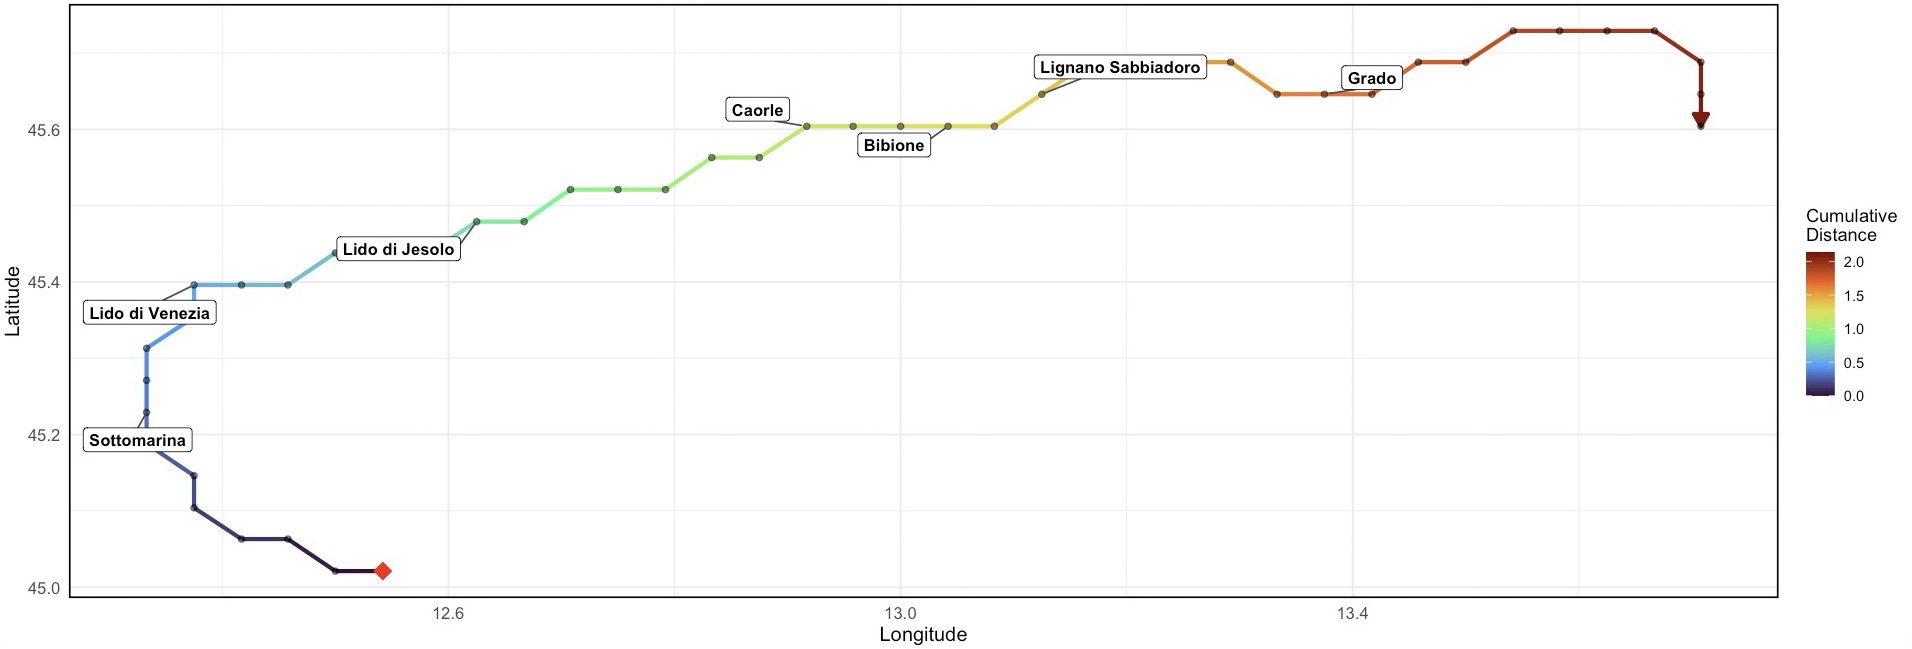
\includegraphics[width=0.8\textwidth]{Images/Coast Linearization copia.jpeg}
    \caption{Spatial linearization of the Northern Adriatic coastline.}
    \label{fig:coast_linearization}
\end{figure}







\newpage
\subsection{Functional Representation (B-Splines with Roughness Penalty)}
\label{subsec:bsplines}

To transform discrete, noisy coastal data into continuous profiles, we employed a \textbf{rich basis} of \textbf{Cubic B-splines} following the P-splines approach \cite{eilers1996flexible}. By placing knots at each measured position along the coast, we capture local features while preventing overfitting through the minimization of the \textbf{Penalized Sum of Squared Errors (PENSSE)}:

$$PENSSE_{\lambda} = \sum_{i=1}^{N} [y_{t,i} - X_t(d_i)]^2 + \lambda \int [X_t''(d)]^2 dd$$

In this formulation, $y_{t,i}$ are raw observations, $X_t(d) = \sum c_{t,k} \phi_k(d)$ is the functional fit, and $\lambda$ is the \textbf{roughness penalty} controlling the curvature (integrated squared second derivative). This approach shifts model complexity from knot placement to the continuous tuning of $\lambda$, effectively filtering measurement noise while preserving macroscopic spatial trends.

\begin{figure}[h!]
    \centering
    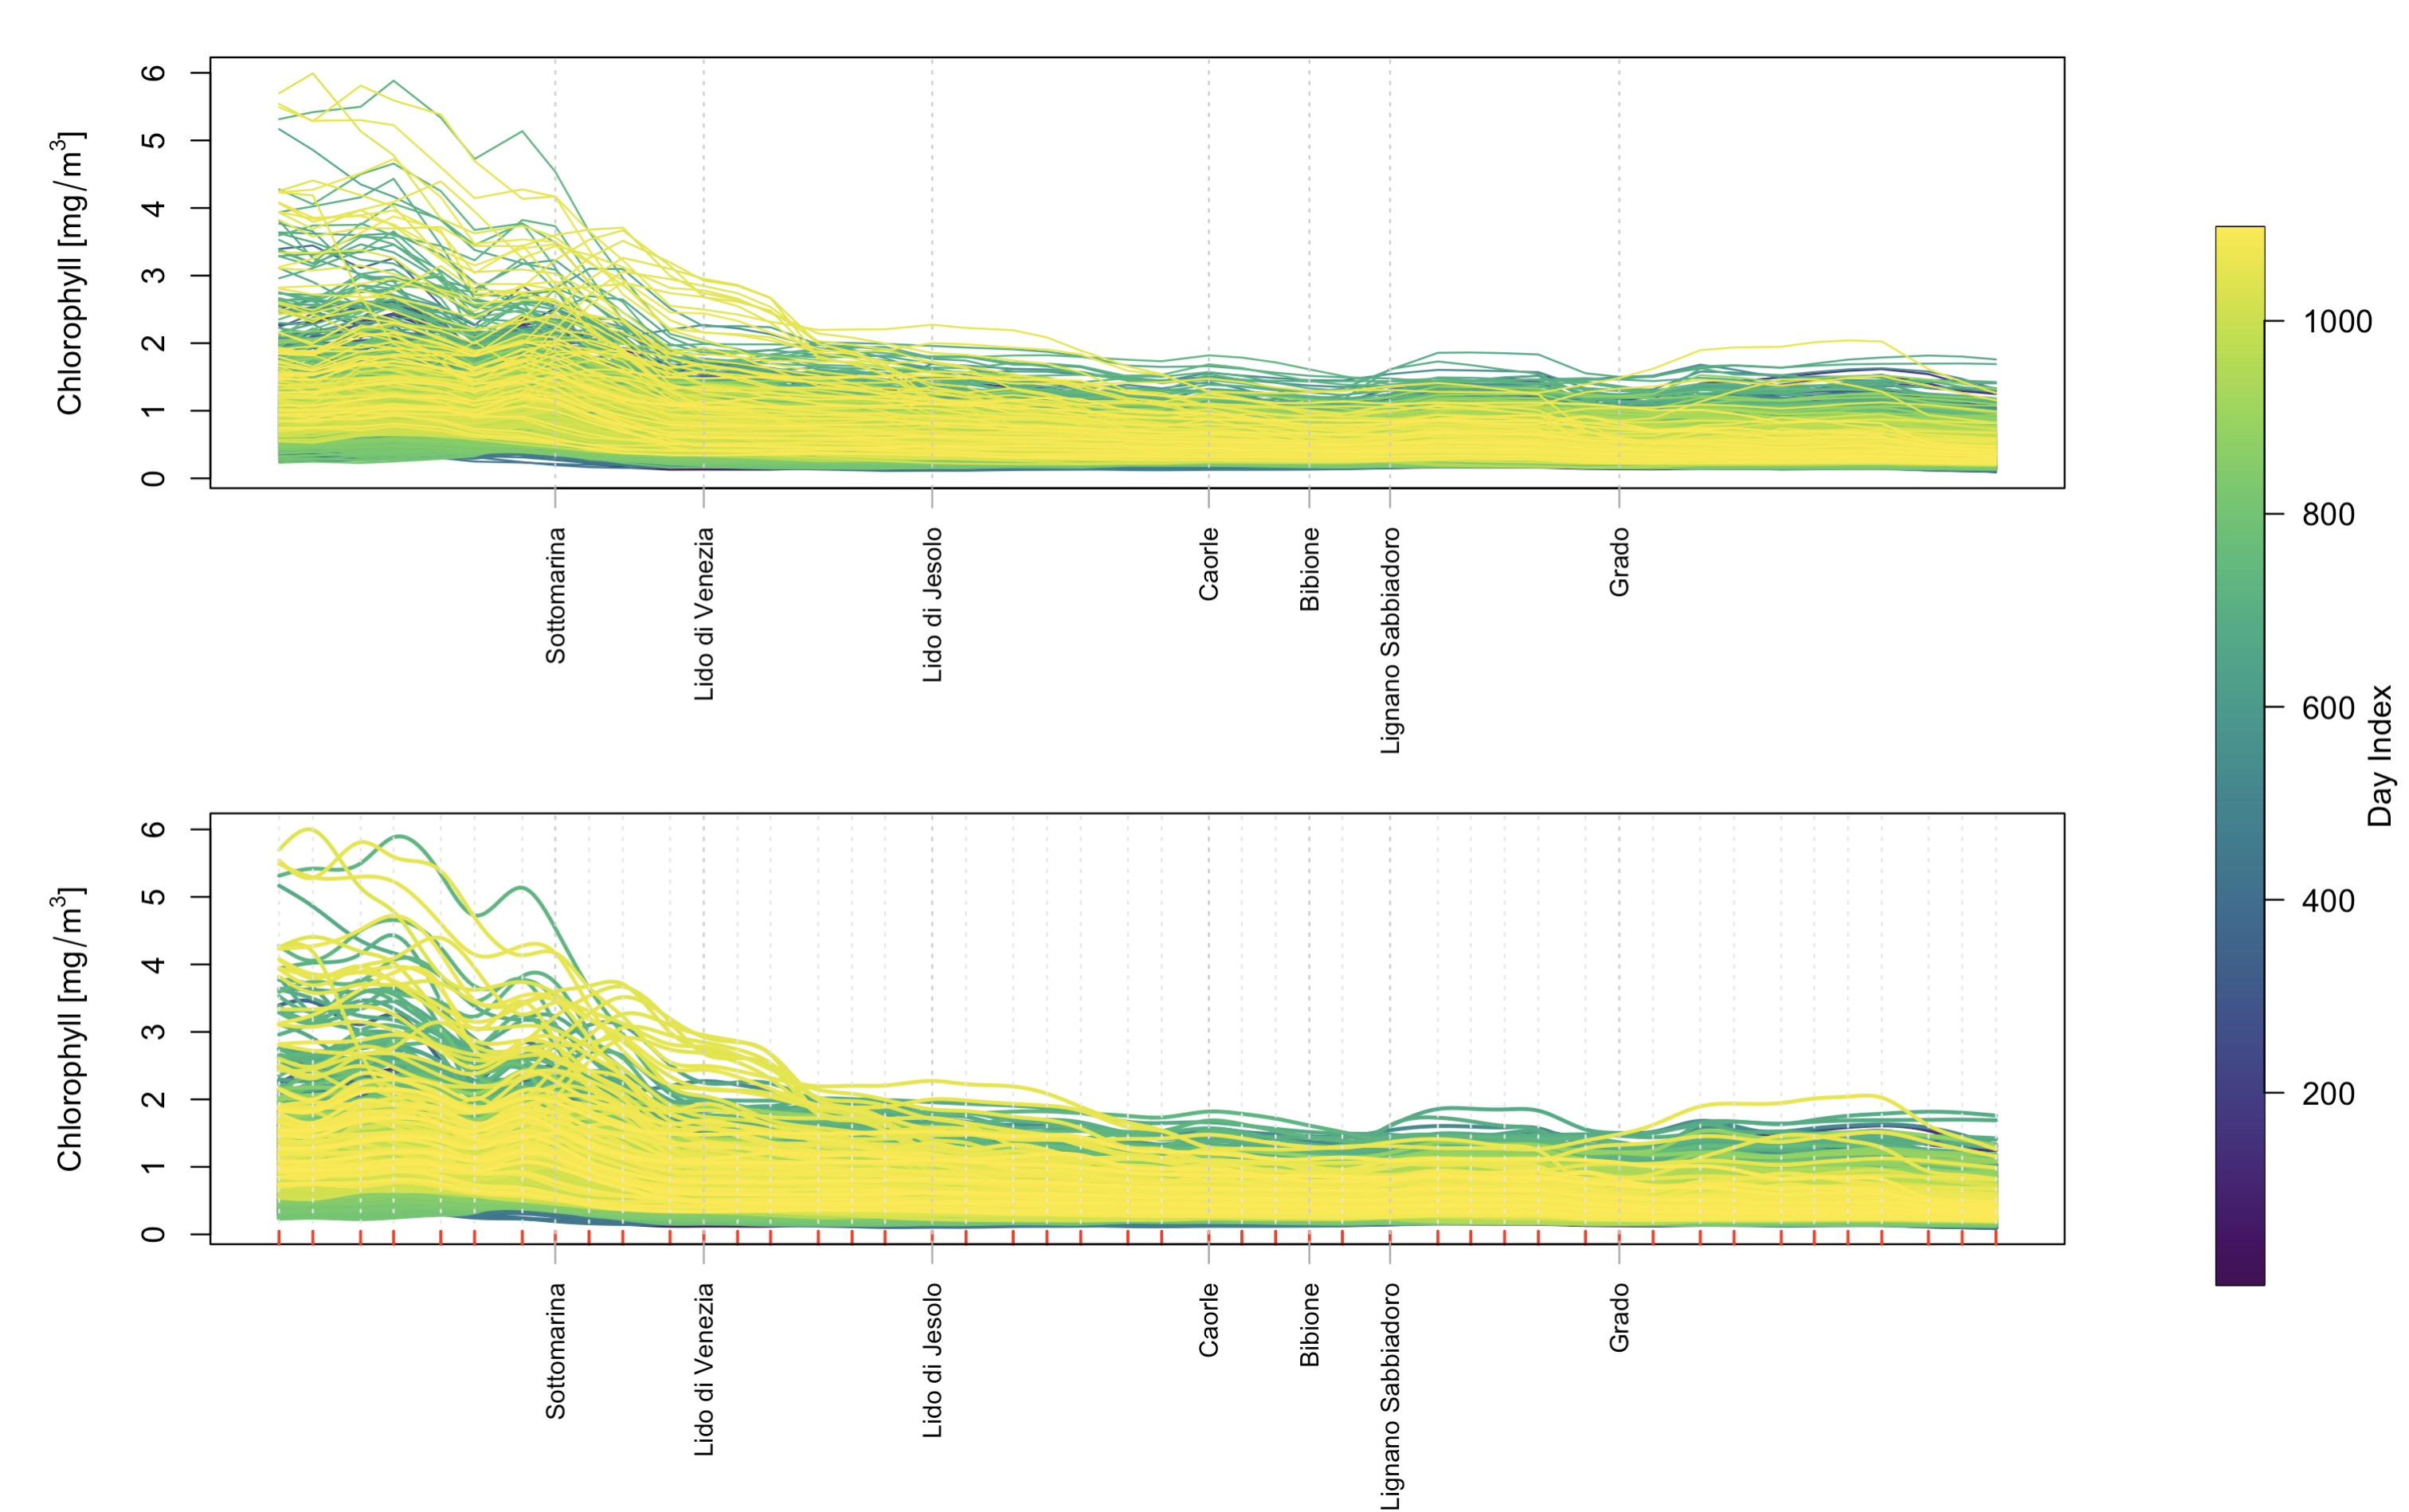
\includegraphics[width=0.8\textwidth]{Images/RAW VS SMOOTHED.jpeg}
    \caption{\textbf{Top:} Raw discrete observations of Chlorophyll-a. \textbf{Bottom:} Continuous functional profiles obtained via B-spline smoothing with penalty $\lambda$.}
    \label{fig:raw_vs_smoothed}
\end{figure}




\subsection{Functional Outlier Detection}
\label{subsec:outliers}

In the context of coastal monitoring, statistical outliers do not represent erroneous data to be discarded, but rather the extreme ecological events (algal blooms) we aim to study.

Functional data allows us to distinguish between two fundamentally different types of anomalies:
\begin{itemize}
    \item \textbf{Magnitude Outliers:} Days where the overall Chlorophyll concentration is abnormally high across the entire coastline. These represent massive, widespread bloom events and are identified using a \textit{Functional Boxplot}.
    \item \textbf{Shape Outliers:} Days where the spatial distribution of Chlorophyll exhibits highly unusual patterns (e.g., severe localized spikes uncharacteristic of the usual North-South gradient). These are identified using the \textit{Outliergram}, a tool based on the relationship between the Modified Banded Depth (MBD) and the Modified Epigraph Index (MEI) \cite{arribas2014shape}.
\end{itemize}

\begin{figure}[h!]
    \centering
    % Prima immagine (Sinistra)
    \begin{minipage}{0.48\textwidth}
        \centering
        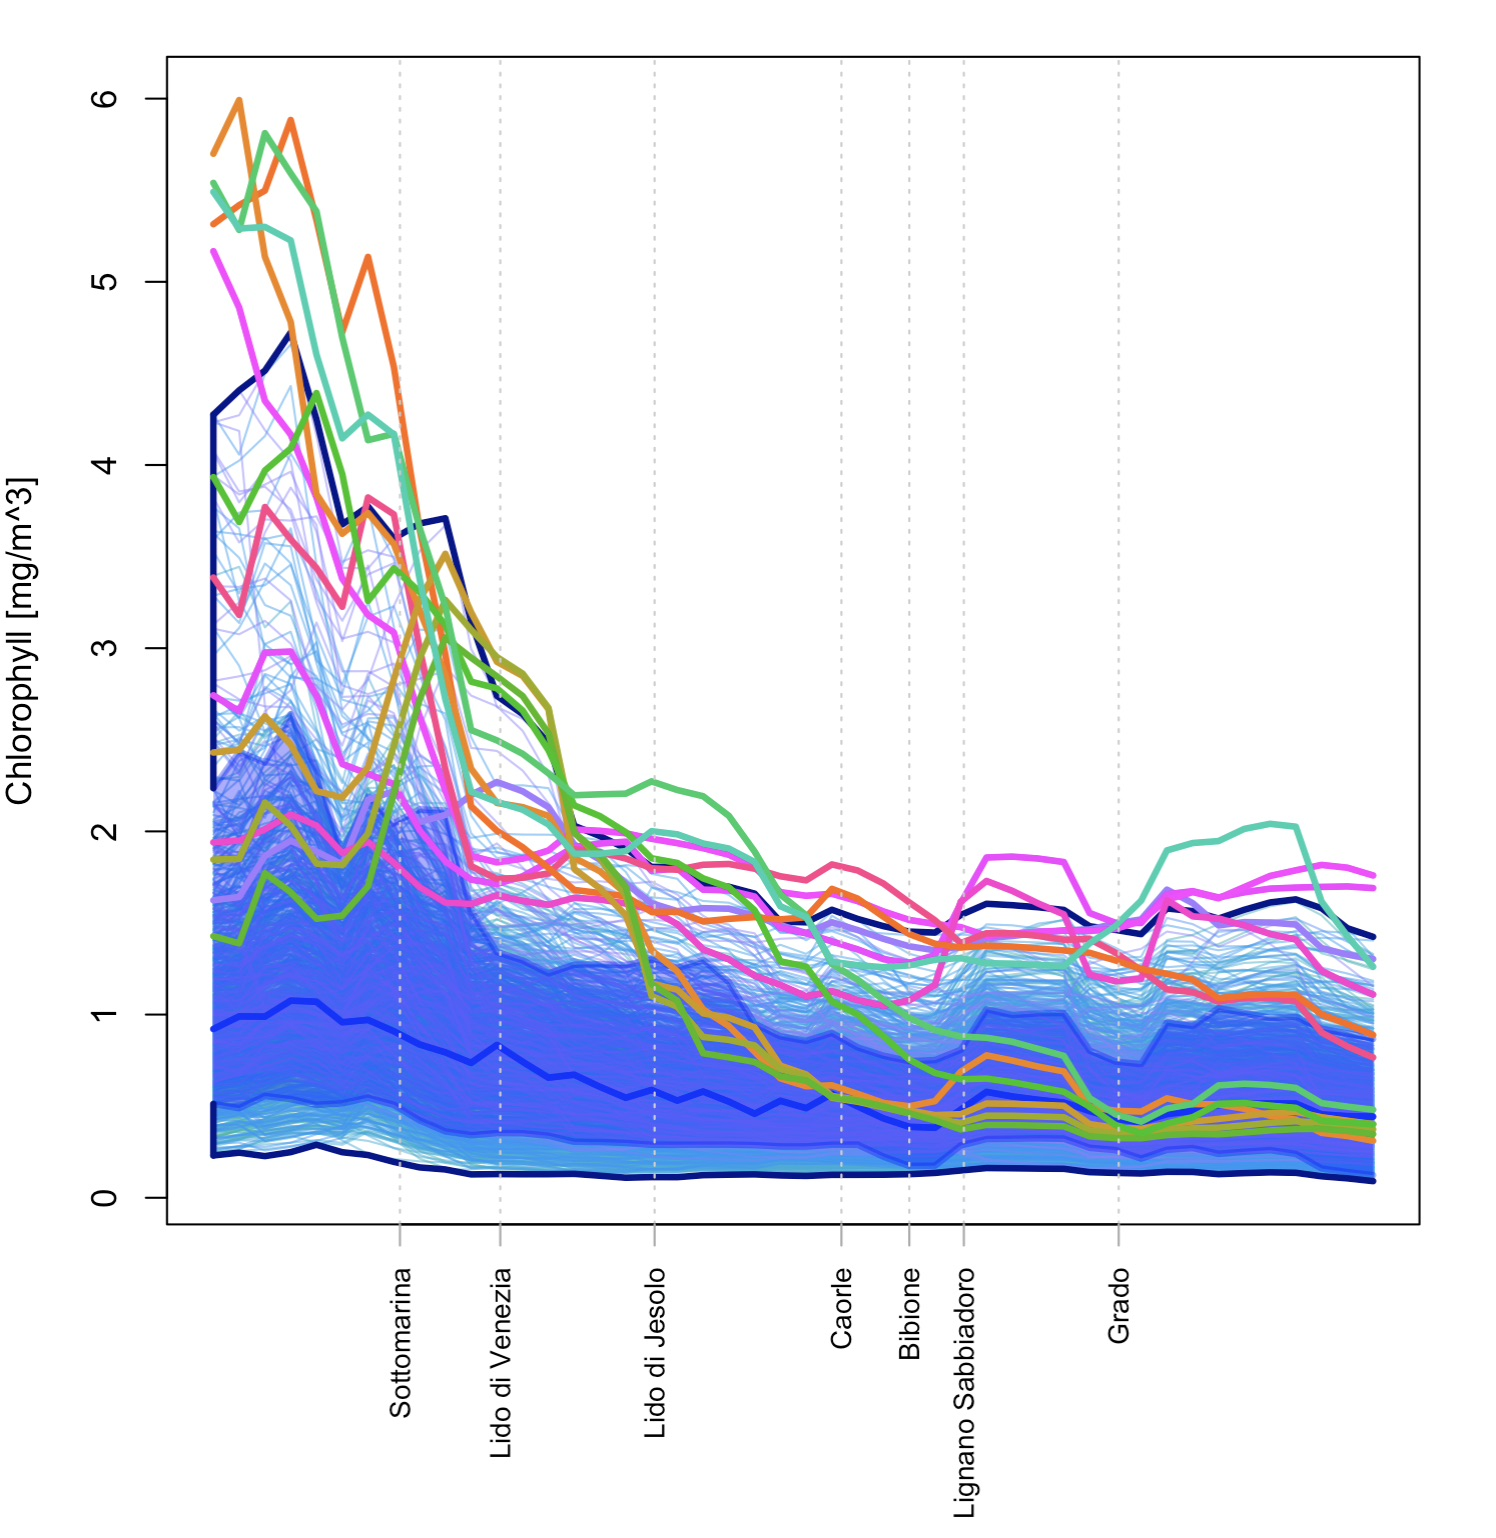
\includegraphics[width=\linewidth]{Images/FUNCTIONAL BOXPLOT senza titolo.jpeg}
        \caption{Functional Boxplot (magnitude outlier detection).}
        \label{fig:boxplot}
    \end{minipage}\hfill
    % Seconda immagine (Destra)
    \begin{minipage}{0.48\textwidth}
        \centering
        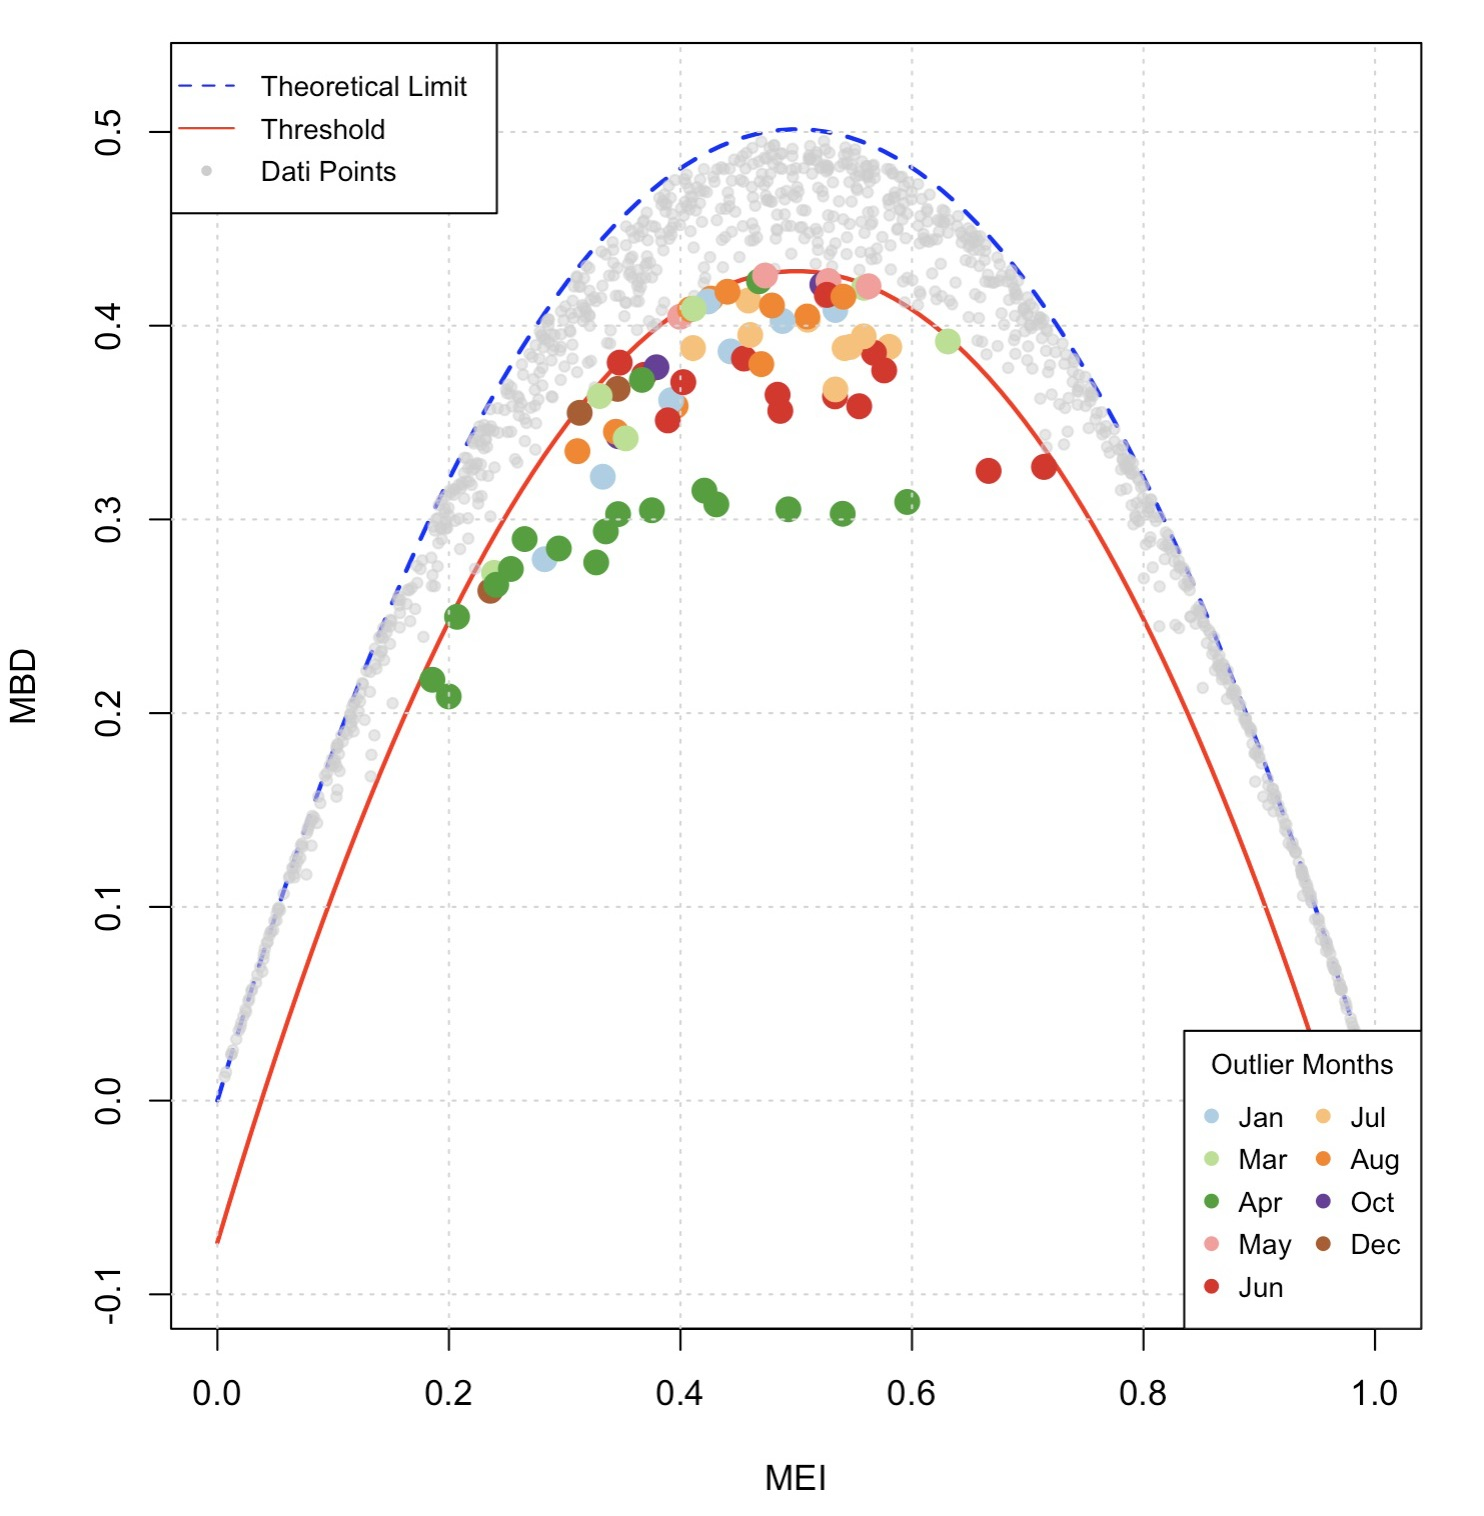
\includegraphics[width=\linewidth]{Images/OUTLIERGRAM senza titolo.jpeg}
        \caption{Outliergram (shape outlier detection).}
        \label{fig:outliergram}
    \end{minipage}
\end{figure}

By extracting the dates corresponding to these anomalies, we aggregated the outliers by month to analyze their temporal distribution.

\begin{figure}[h!]
    \centering
    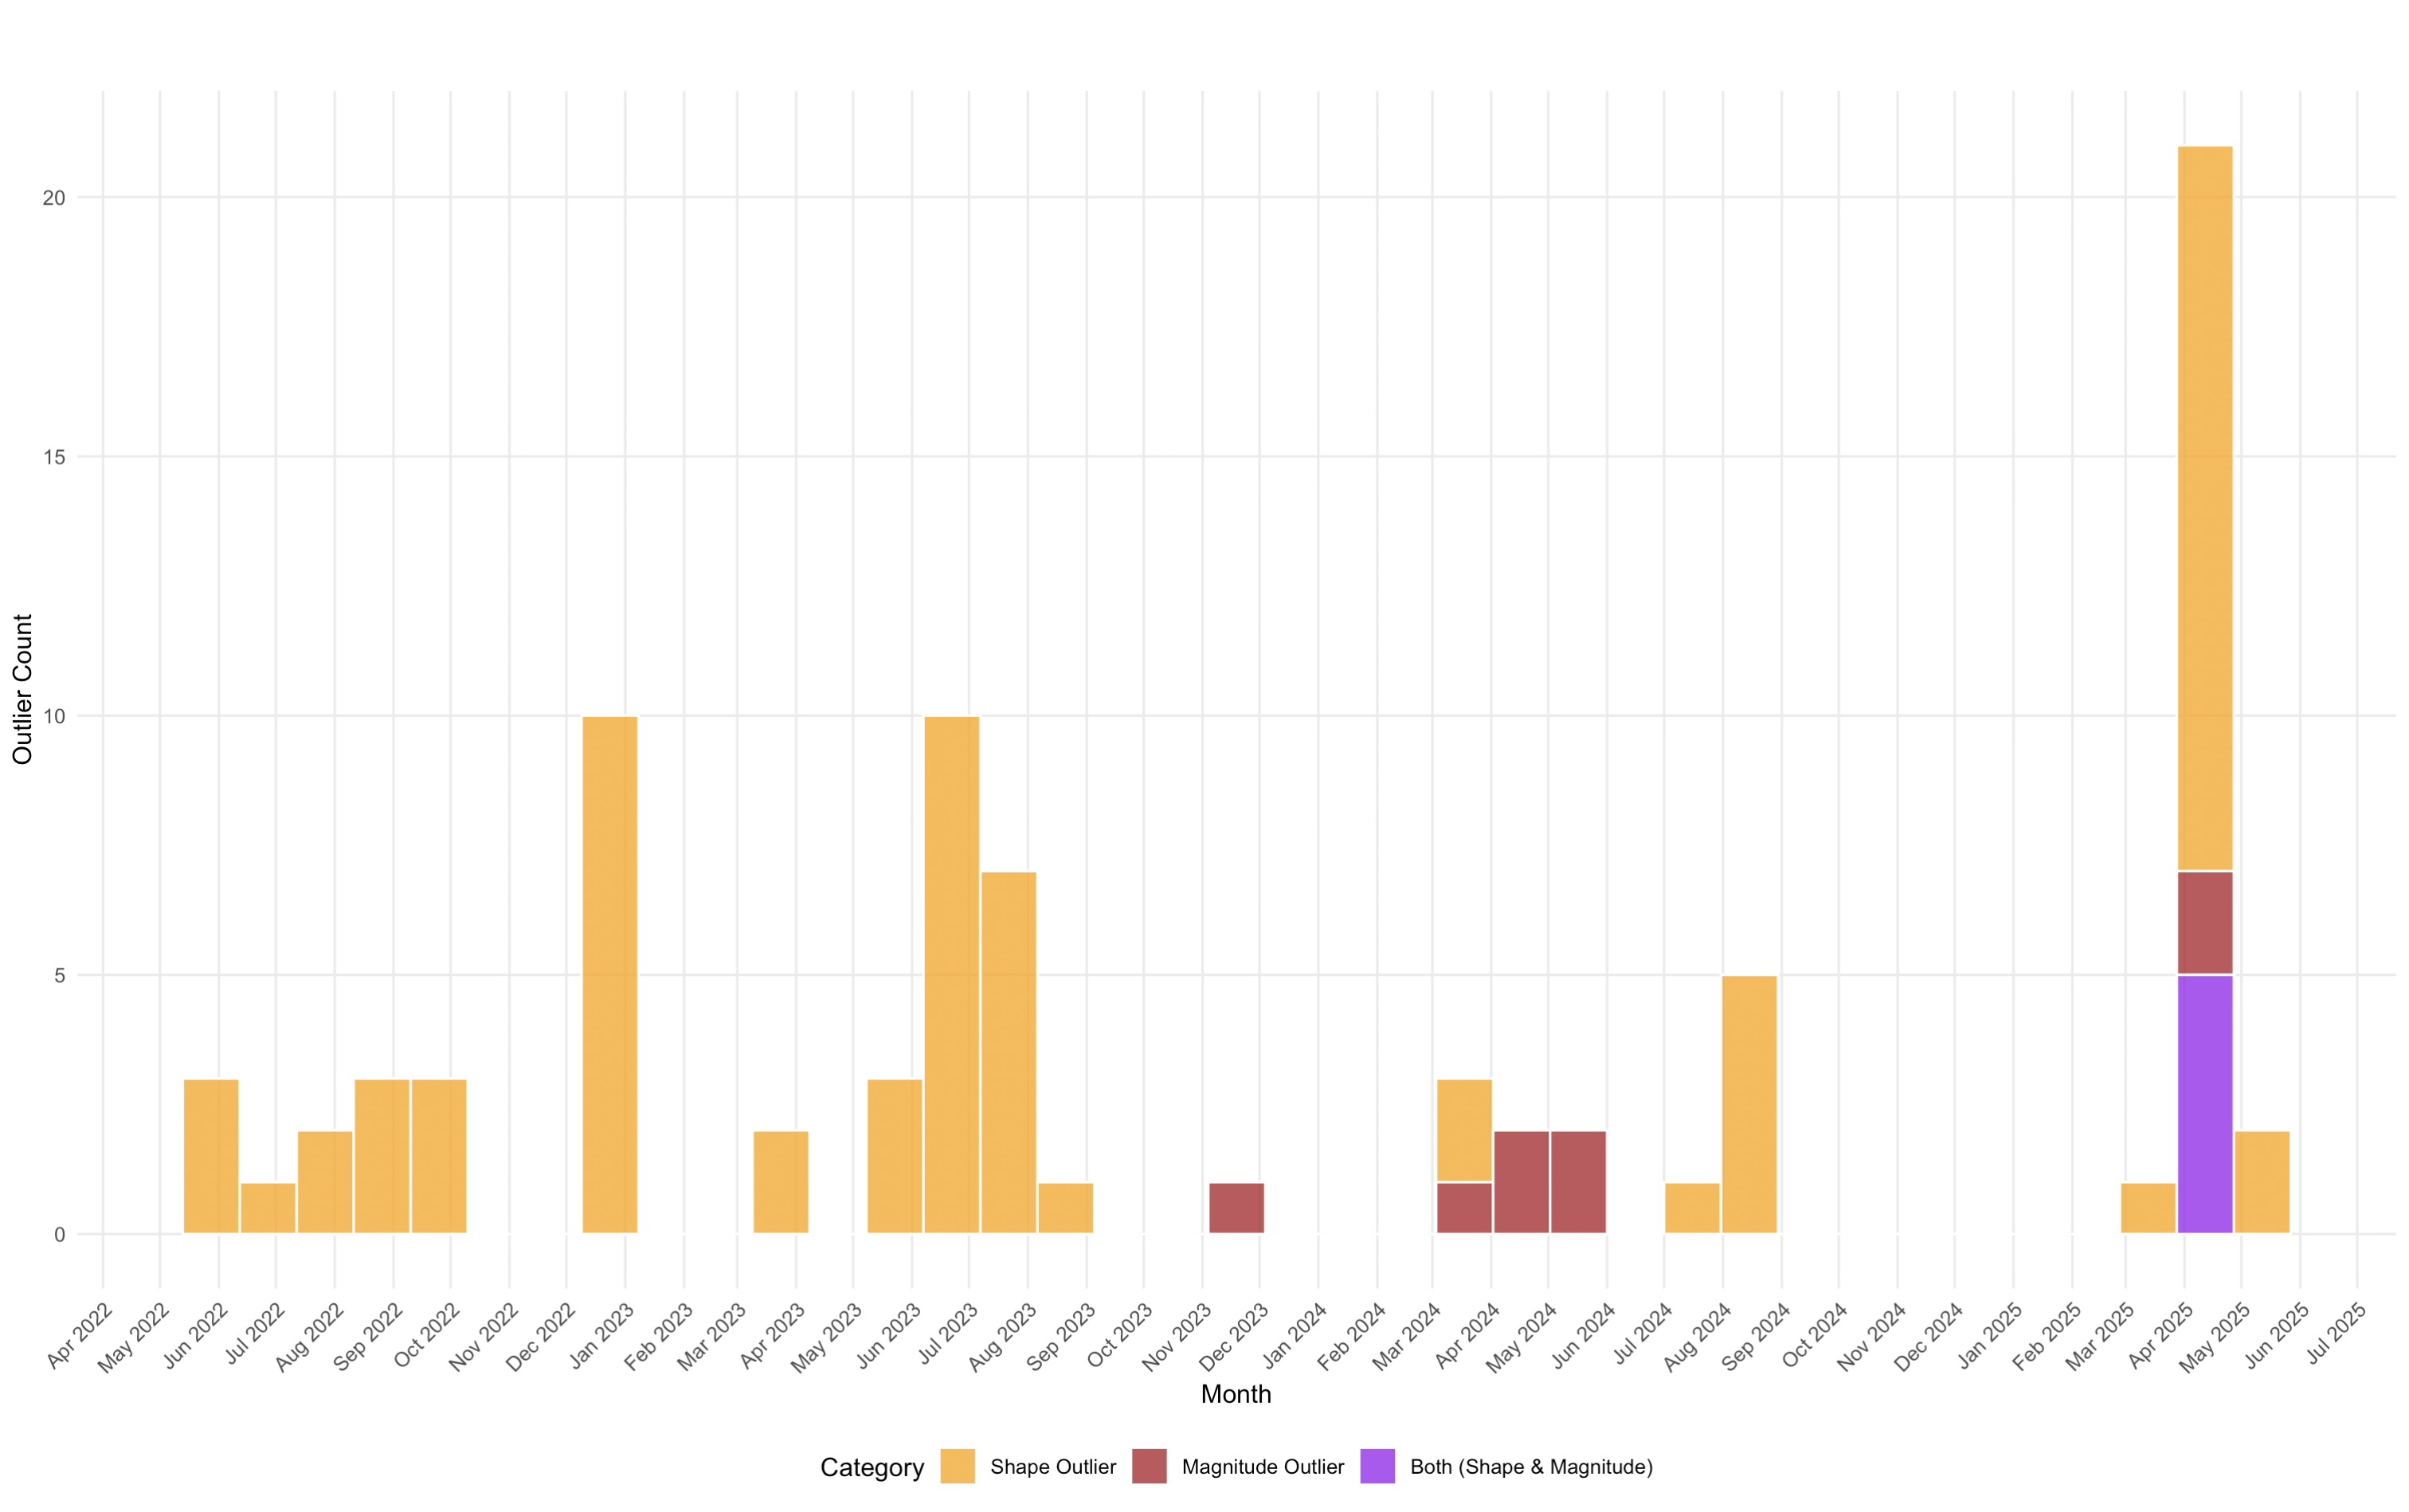
\includegraphics[width=0.8\textwidth]{Images/MONTHLY FREQUENCY OUTLIERS senza titolo.jpeg}
    \caption{Monthly distribution of dagnitude and shape outliers.}
    \label{fig:monthly_outliers}
\end{figure}

The monthly frequency analysis reveals critical patterns for \textit{Meteo.Adriatico}. Specifically, we observed that shape outliers rarely exceed 5 occurrences per month (out of approximately 30 daily profiles). While a slight increase in shape anomalies was noted in January and during the summer of 2023, the monthly count never surpassed 10. Magnitude outliers are exceptionally rare, with just over ten instances recorded across the entire three-year dataset. This confirms that Chlorophyll dynamics predominantly follow smooth, regular seasonal patterns without erratic fluctuations. The only major exception occurred in April 2025, which registered a significant anomaly of 21 total outliers (5 exhibiting both magnitude and shape anomalies, 2 magnitude-only, and 14 shape-only). Ultimately, while functional anomalies are present and ecologically relevant, their overall low frequency ensures they do not introduce disruptive noise or invalidate the robust forecasting architectures developed in this study.



\subsection{Dimensionality Reduction via FPCA}
Modeling the full functional curves directly proved computationally prohibitive for iterative forecasting algorithms. To efficiently reduce dimensionality without sacrificing critical information, we applied \textbf{Functional Principal Component Analysis (FPCA)}. FPCA decomposes the functional variance into orthogonal modes of variation:
$$X_t(d) = \mu(d) + \sum_{j=1}^{J} \xi_{t,j} \psi_j(d)$$
    where $\mu(d)$ is the mean functional profile, $\psi_j(d)$ are the functional principal components (FPCs) representing the dominant spatial patterns, and $\xi_{t,j}$ are the principal component scores. Our analysis revealed that the first 4 components explain over $96\%$ of the total spatial variance. 

\begin{figure}[h!]
    \centering
    \begin{minipage}{0.35\textwidth}
        \centering
        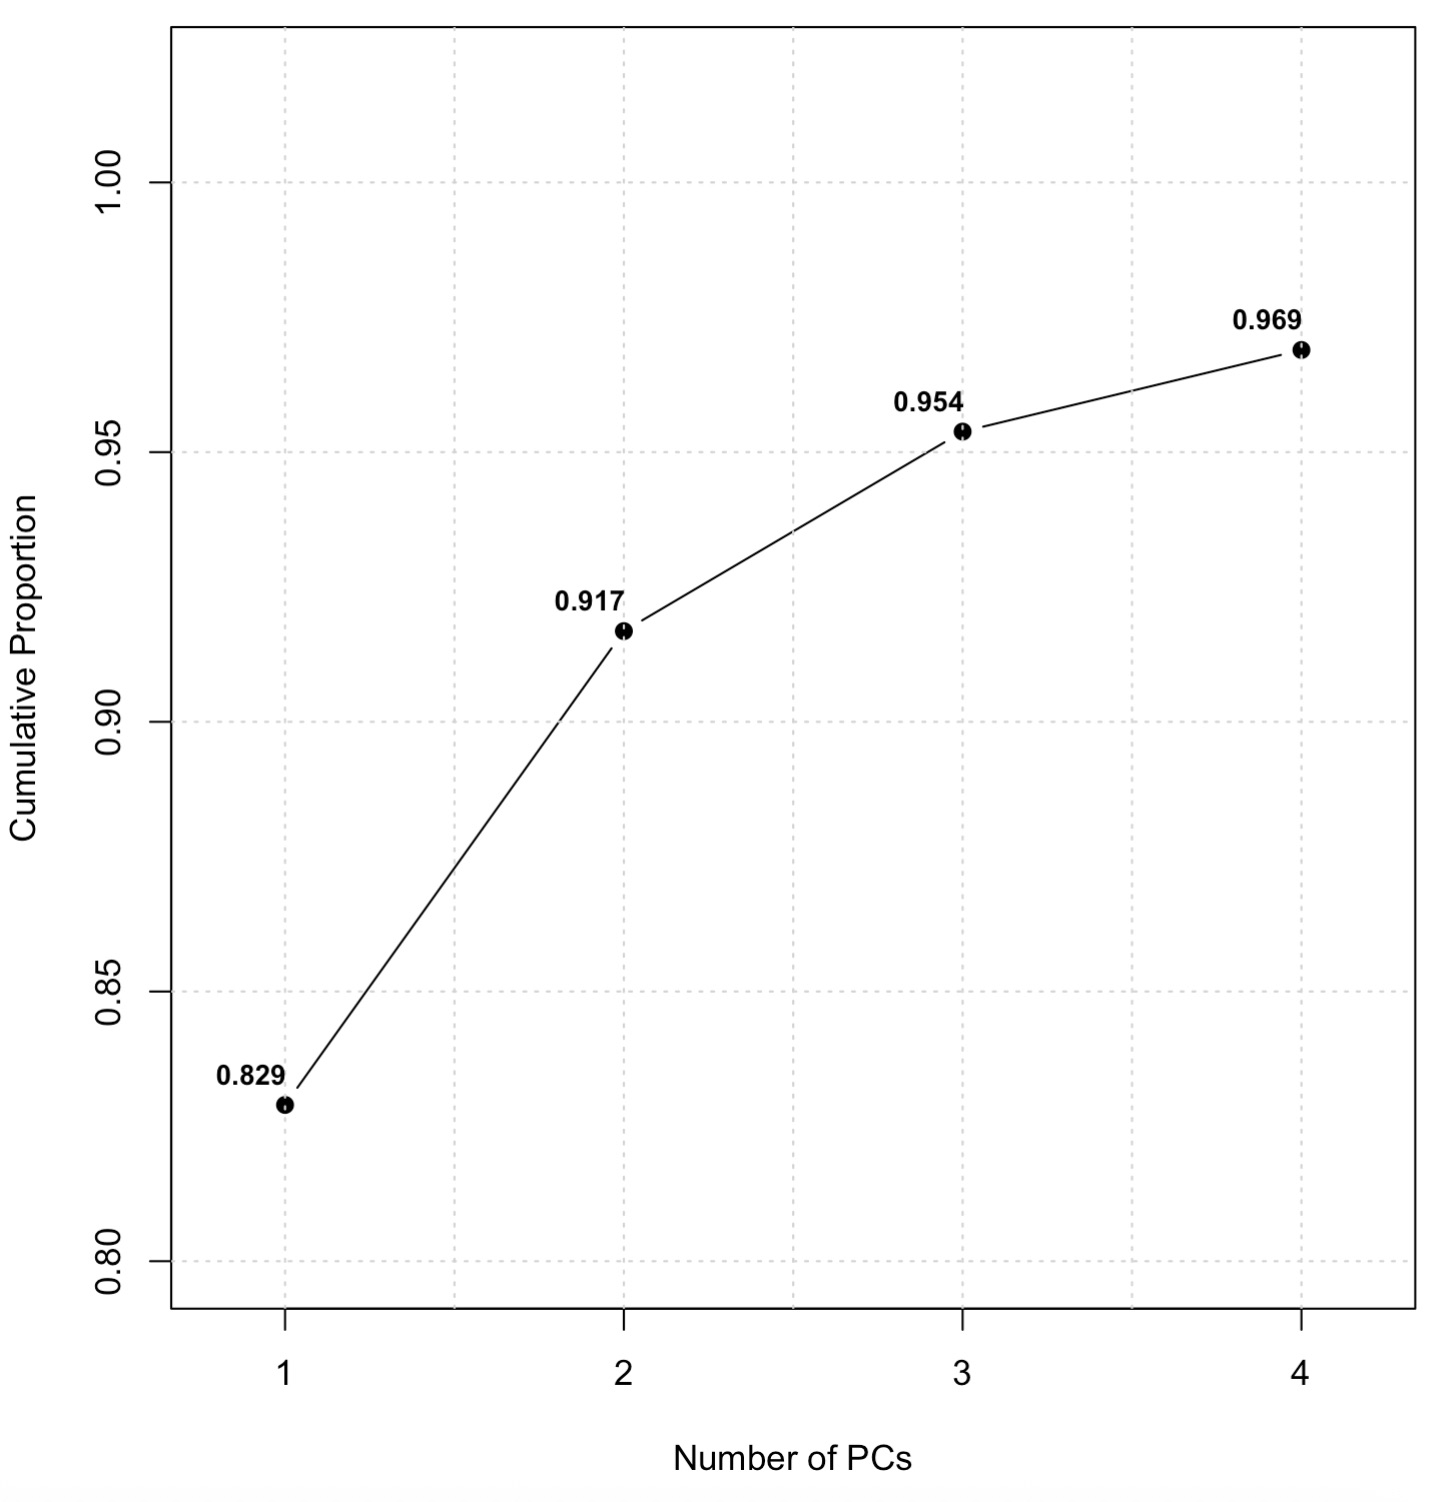
\includegraphics[width=\linewidth]{Images/FPCA Scree Plot senza titolo.jpeg}
        \caption{FPCA scree plot.}
        \label{fig:fpca_scree}
    \end{minipage}\hfill
    \begin{minipage}{0.62\textwidth}
        \centering
        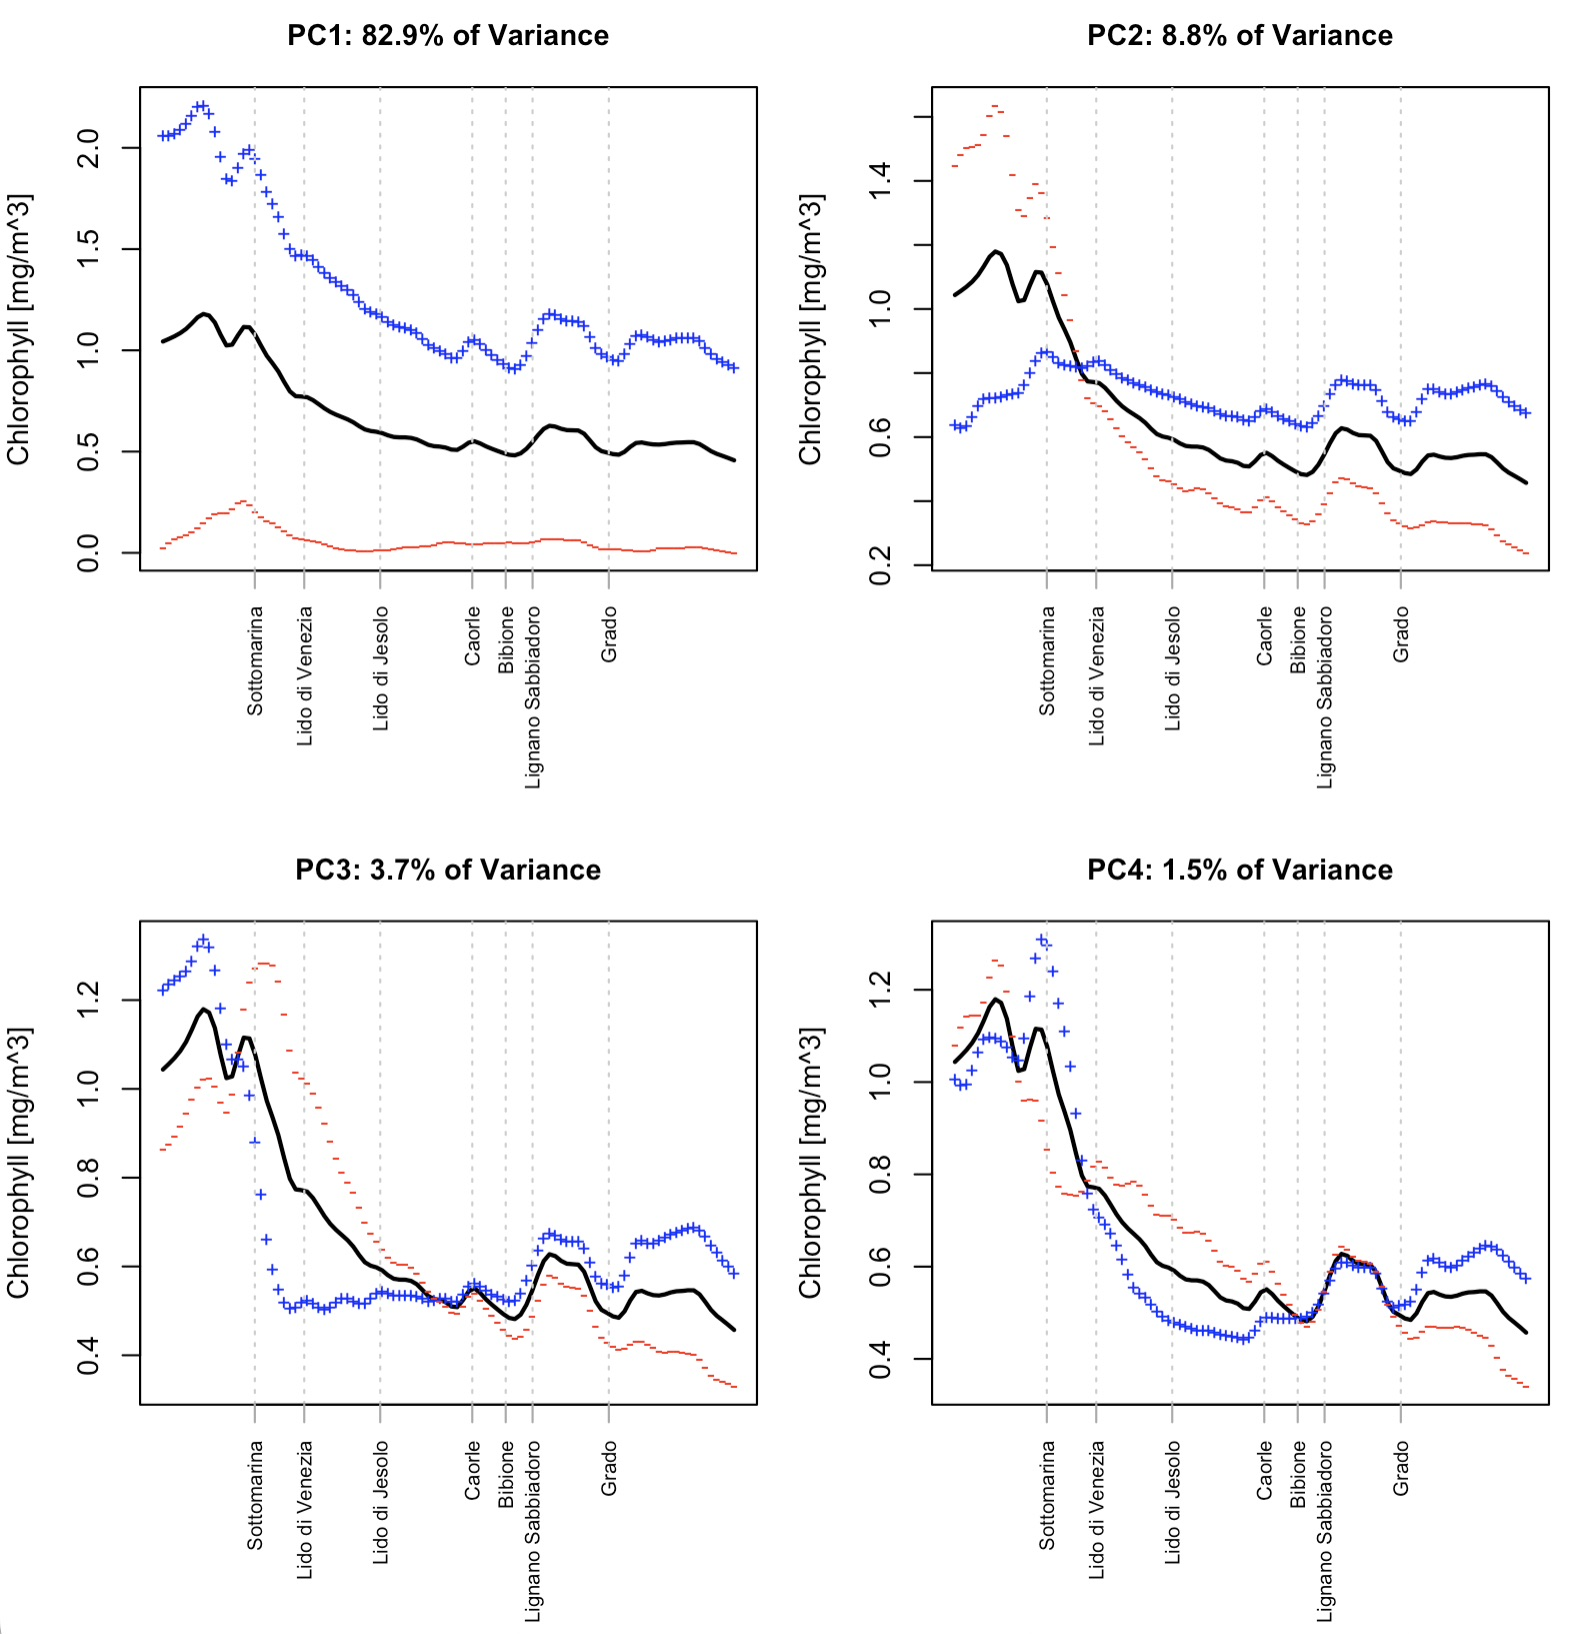
\includegraphics[width=\linewidth]{Images/PCs VISUALIZATION diverso.jpeg}
        \caption{First four principal components ($\psi_j$).}
        \label{fig:fpca_pcs}
    \end{minipage}
\end{figure}

The interpretation of these spatial modes is shown in Figure \ref{fig:fpca_pcs}. Specifically, $\psi_1$ acts as a \textit{magnitude operator}: the mean profile (black) lies between the positive (blue) and negative (red) variations, meaning a high score $\xi_{t,1}$ indicates a generalized increase in Chlorophyll across the coast. $\psi_2$ captures \textit{spatial redistribution}, contrasting flatter profiles with those showing extreme fluctuations at the coastal boundaries. Finally, $\psi_3$ and $\psi_4$ represent higher-order spatial residuals of more complex interpretation.

To ensure our framework adapts to seasonal and structural changes in the Adriatic ecosystem, we implemented a \textbf{rolling window methodology}. The FPCA basis is calculated using a training set comprising the 365 days prior to the forecast date. This basis is updated daily, allowing the model to incorporate the most recent oceanographic trends. 

Our forecasting models target the evolution of the principal component scores for the upcoming 7 days. Once predicted, these scores ($\hat{\xi}_{t+h,j}$) are used to reconstruct the full functional Chlorophyll profile. 

\begin{figure}[h!]
    \centering
    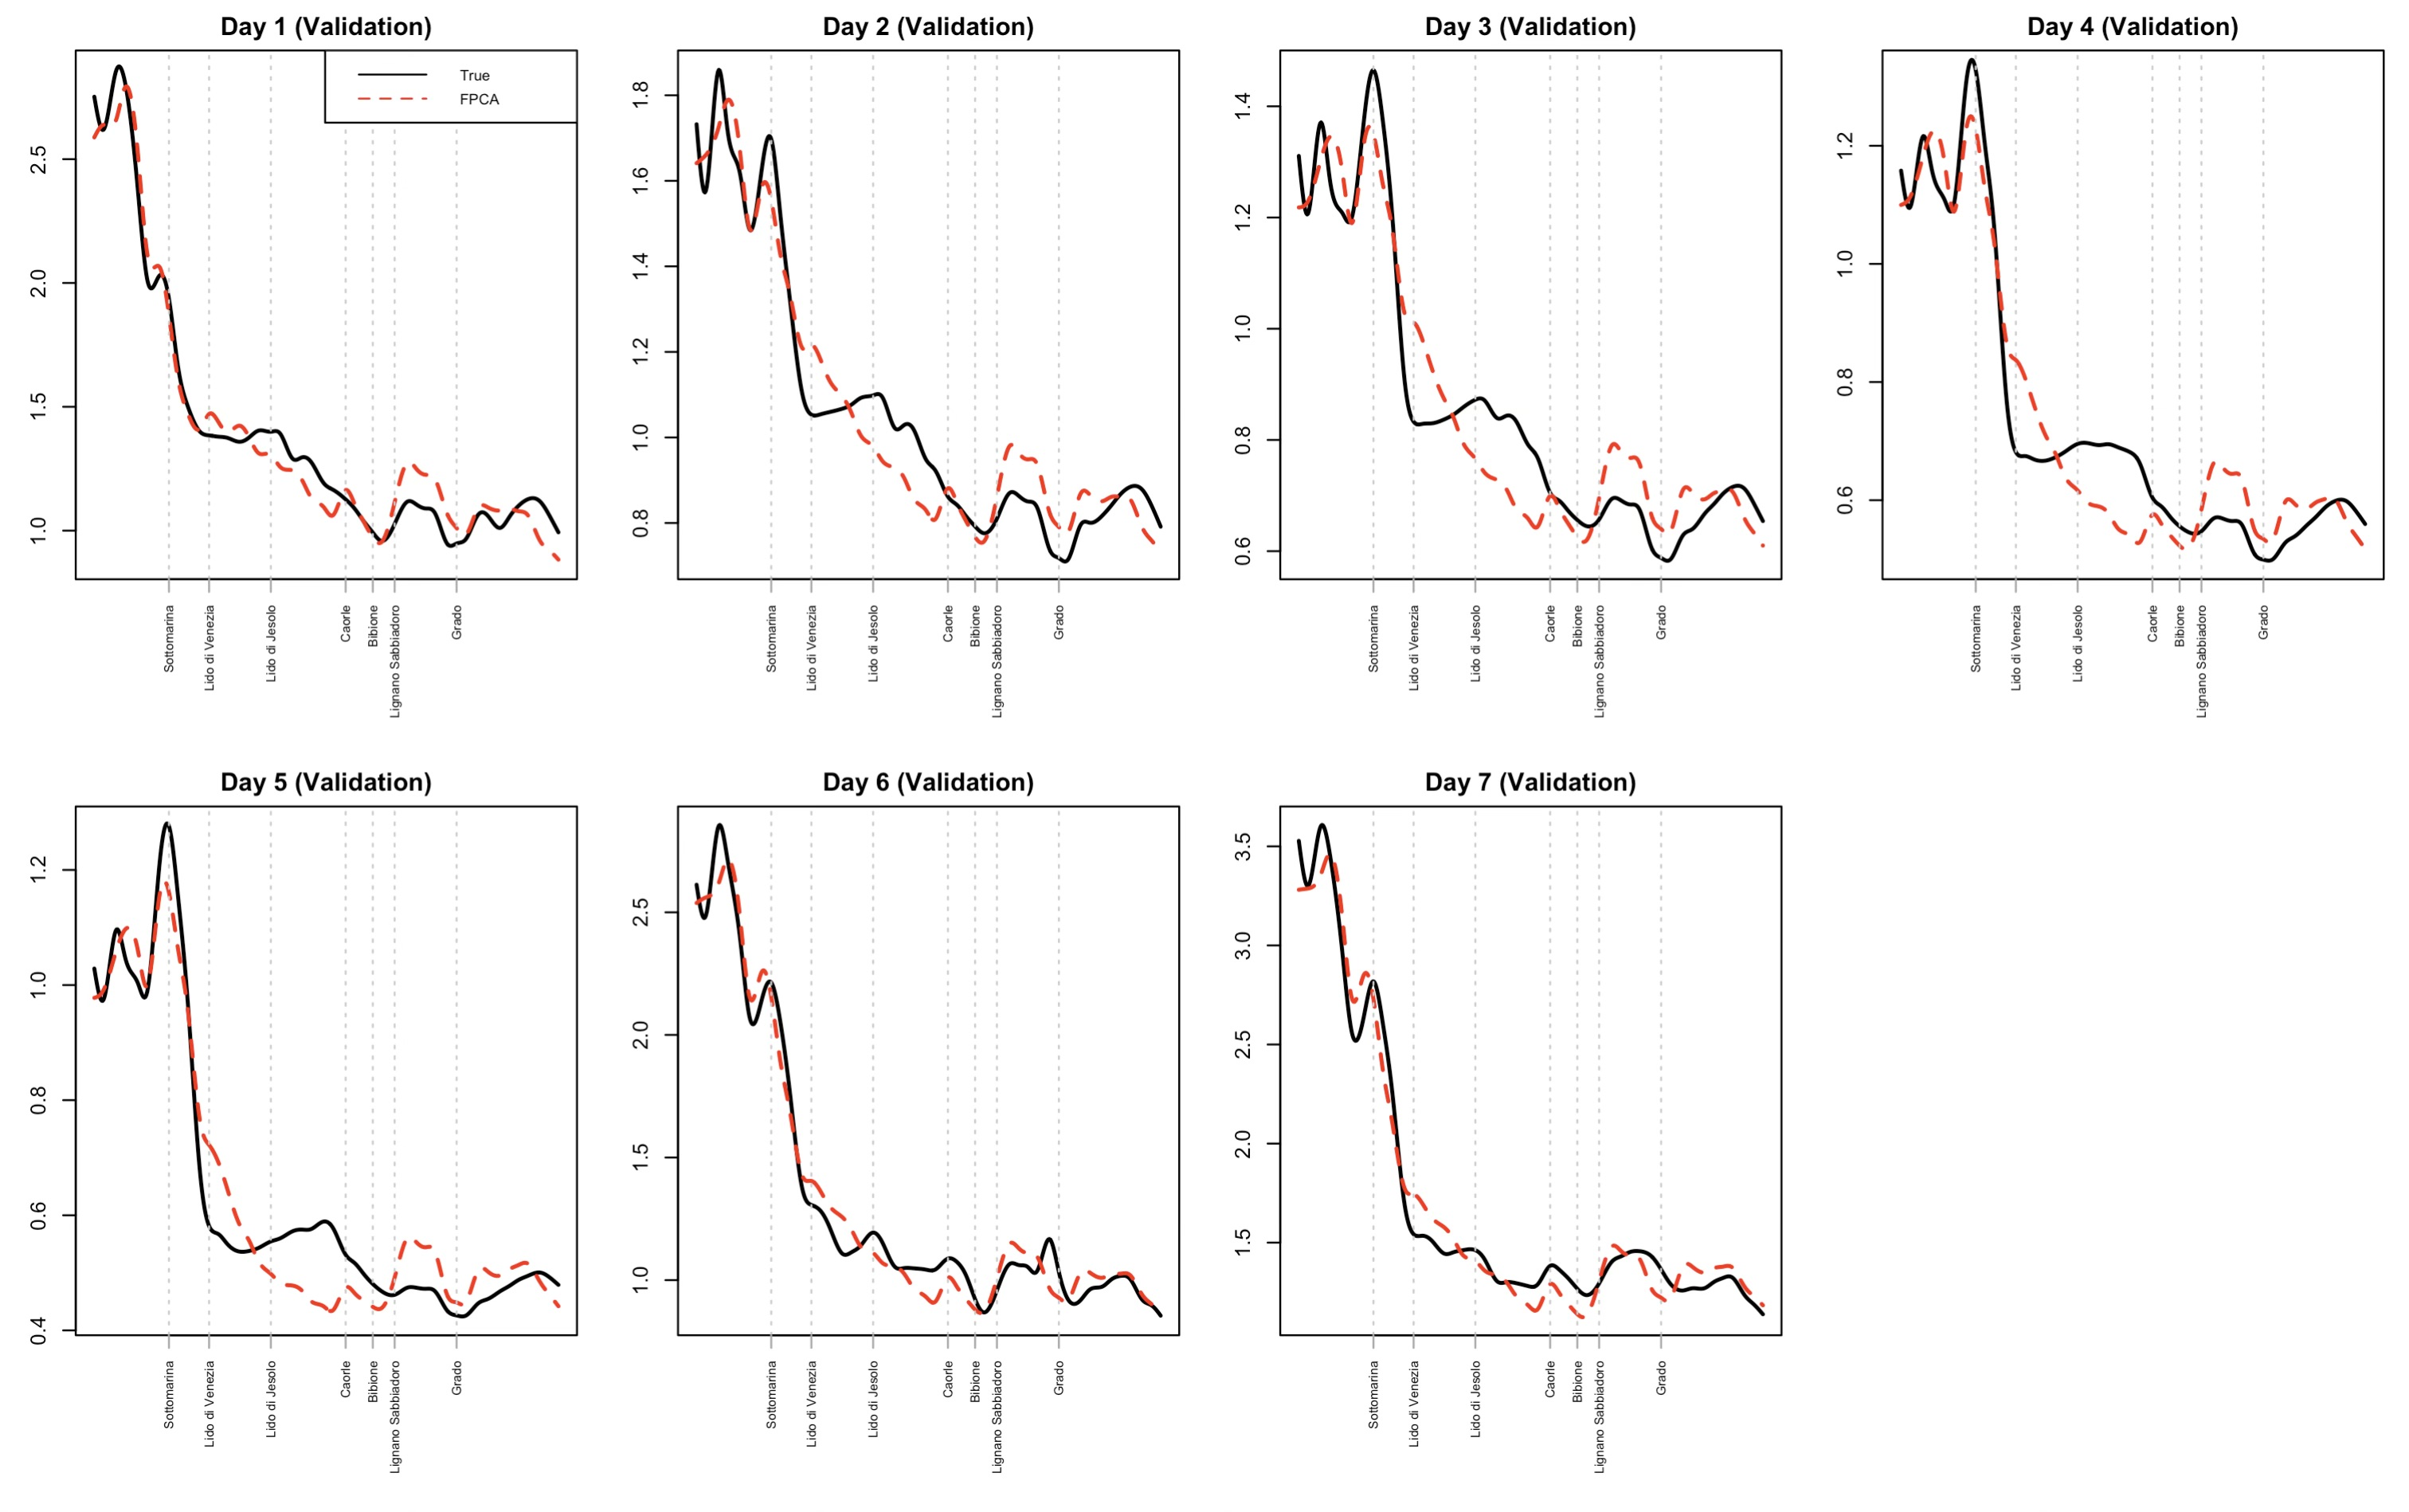
\includegraphics[width=0.85\textwidth]{Images/Reconstruction validation.jpeg}
    \caption{Validation of the reconstruction method.}
    \label{fig:reconstruction_val}
\end{figure}

The effectiveness of this reconstruction is demonstrated in Figure \ref{fig:reconstruction_val}, which compares observed profiles with curves reconstructed from forecasted scores over a one-week horizon. The results show that the reconstruction effectively captures the macroscopic spatial dynamics, validating our dimensionality reduction approach for operational forecasting.
















\clearpage
\newpage
\section{Forecasting Strategies and Model Comparison}
\label{sec:forecasting}
After projecting the functional data onto the first 4 Principal Components (explaining $\approx 96\%$ of total variance), the forecasting task was reduced to a multivariate time-series problem. We aimed to predict the future score vectors $\boldsymbol{\xi}_{t+h}$ based on their historical trajectories. To identify the most robust approach, we conducted a comparative analysis of four distinct modeling strategies.

\subsection{Candidate Models}
\begin{itemize}
    \item \textbf{Vector Autoregression (VAR):} We implemented a VAR model to capture the linear interdependencies between the four principal components. The underlying hypothesis is that the spatial modes of Chlorophyll distribution are dynamically coupled \cite{ghani2007modelling}.
    \item \textbf{Vector Error Correction Model (VECM):} Since biological time series often exhibit common stochastic trends, we tested for cointegration using the \textit{Johansen Test}. The test indicated the presence of stable long-term relationships (rank $r=3$), motivating the use of VECM to model both short-term dynamics and long-term equilibrium adjustments\cite{hamilton1994time}.
    \item \textbf{eXtreme Gradient Boosting (XGBoost):} To account for potential non-linearities, such as threshold effects typical of algal blooms, we trained an XGBoost regressor. We structured the dataset using a sliding window approach with lagged features ($p=7$ days), allowing the decision trees to learn complex interactions between past and future states\cite{kim2022development}.
    \item \textbf{Benchmark (SARIMA):} We tested a univariate SARIMA model for each principal component to assess if treating them independently (ignoring spatial cross-correlations) would suffice as a simpler baseline\cite{hyndman2018forecasting}.
\end{itemize}

\subsection{Performance Evaluation and Results}

To evaluate the physical accuracy of our forecasts, the predicted component scores ($\hat{\boldsymbol{\xi}}_{t+h}$) were projected back into the original functional space to reconstruct the expected Chlorophyll profiles. We achieved this by multiplying the predicted scores by the fixed FPCA harmonics derived from the training set and adding back the functional mean:
$$\hat{X}_{t+h}(d) = \mu(d) + \sum_{j=1}^{4} \hat{\xi}_{t+h,j} \psi_j(d)$$
This reconstruction step yields a continuous predicted curve for each day of the validation period, which can be visually and metrically compared against the true observed Chlorophyll profiles.

\begin{figure}[h!]
    \centering
    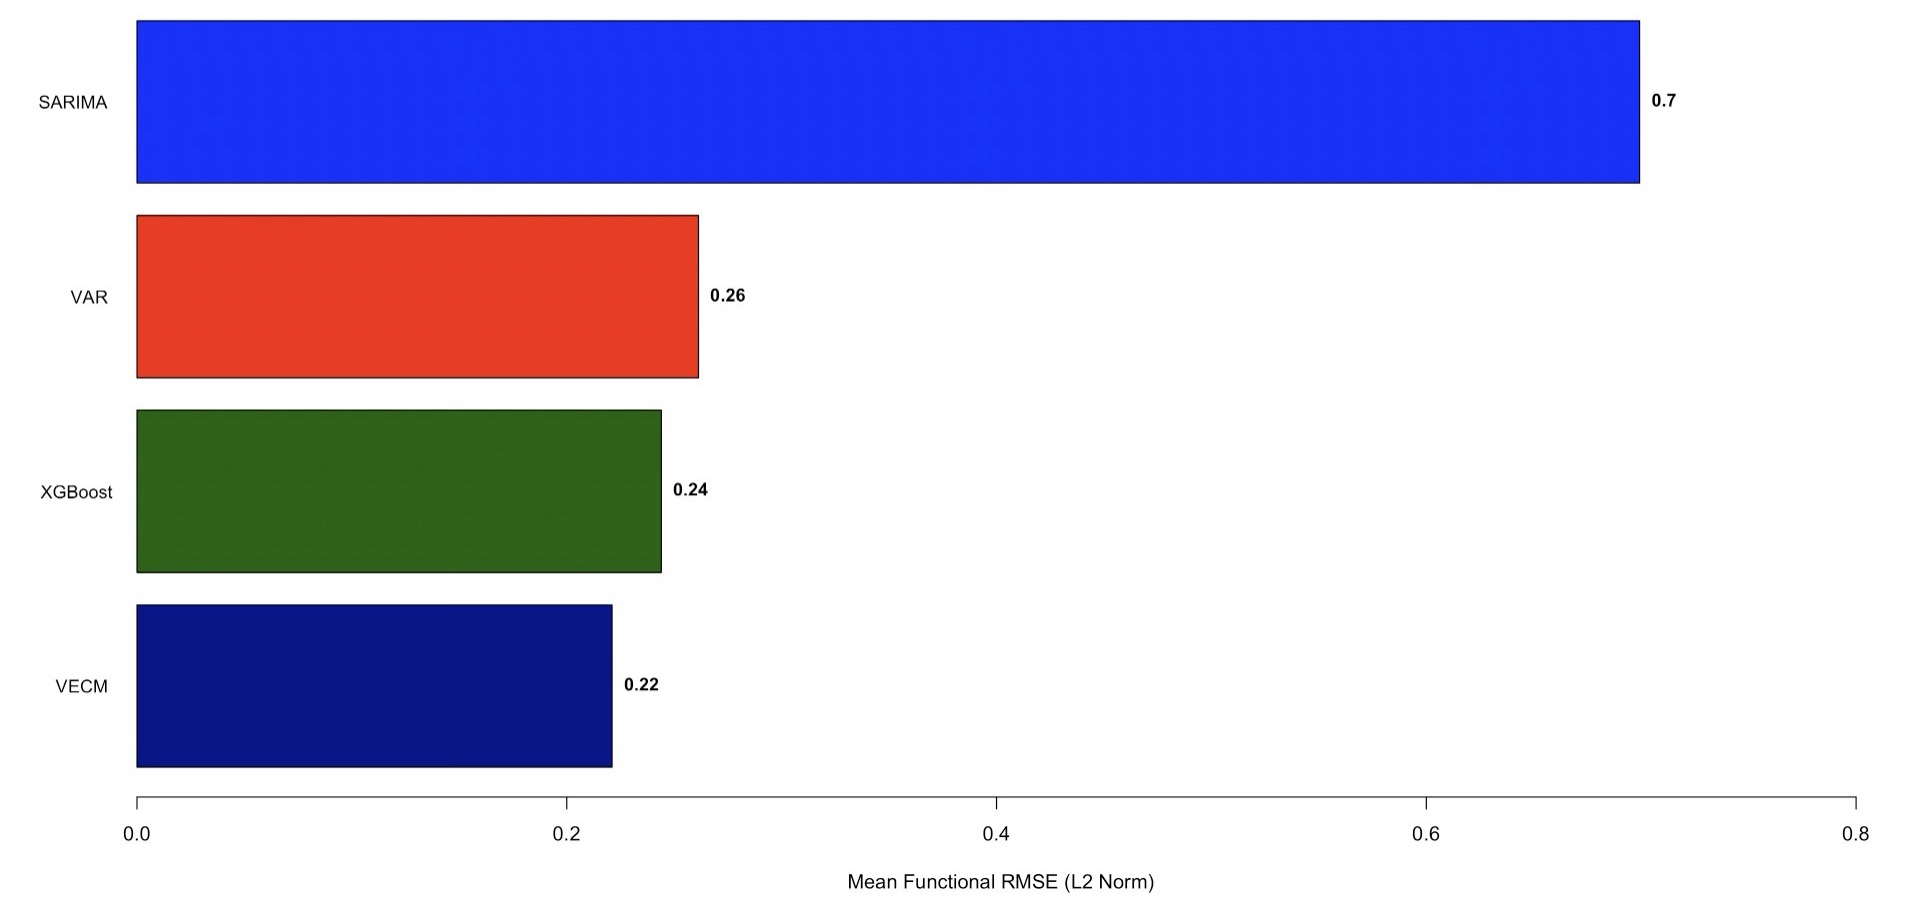
\includegraphics[width=0.8\textwidth]{Images/Barplot RMSE senza titolo.jpeg}
    \caption{RMSE barplot of the four candidate models.}
    \label{fig:RMSE}
\end{figure}

The models were quantitatively evaluated using the \textbf{Mean Functional RMSE} (L2 Norm) over a held-out validation set of $n=7$ days. The final comparison revealed a clear hierarchy in predictive performance:

\begin{enumerate}
    \item \textbf{VECM:} The Vector Error Correction Model achieved the lowest overall error (\textbf{RMSE $\approx 0.22$}). The Johansen test indicated a cointegration rank of $r=3$, confirming that the spatial components share strong long-term stochastic trends. Modeling this equilibrium adjustment proved highly effective for short-term prediction.
    \item \textbf{XGBoost:} The recursive machine learning approach performed competitively (\textbf{RMSE $\approx 0.24$}). Its ability to capture non-linear relationships across lags makes it a robust alternative, although its recursive nature can compound errors over longer horizons.
    \item \textbf{VAR:} The standard Vector Autoregression ranked third (\textbf{RMSE $\approx 0.26$}). While it captures the cross-correlation between spatial modes, the lack of long-term equilibrium constraints makes it slightly less accurate than the VECM.
    \item \textbf{SARIMA:} The univariate approach performed significantly worse (\textbf{RMSE $\approx 0.70$}), definitively proving that treating the spatial components independently, ignoring their dynamic interactions, leads to severe information loss.
\end{enumerate}

\begin{figure}[h!]
    \centering
    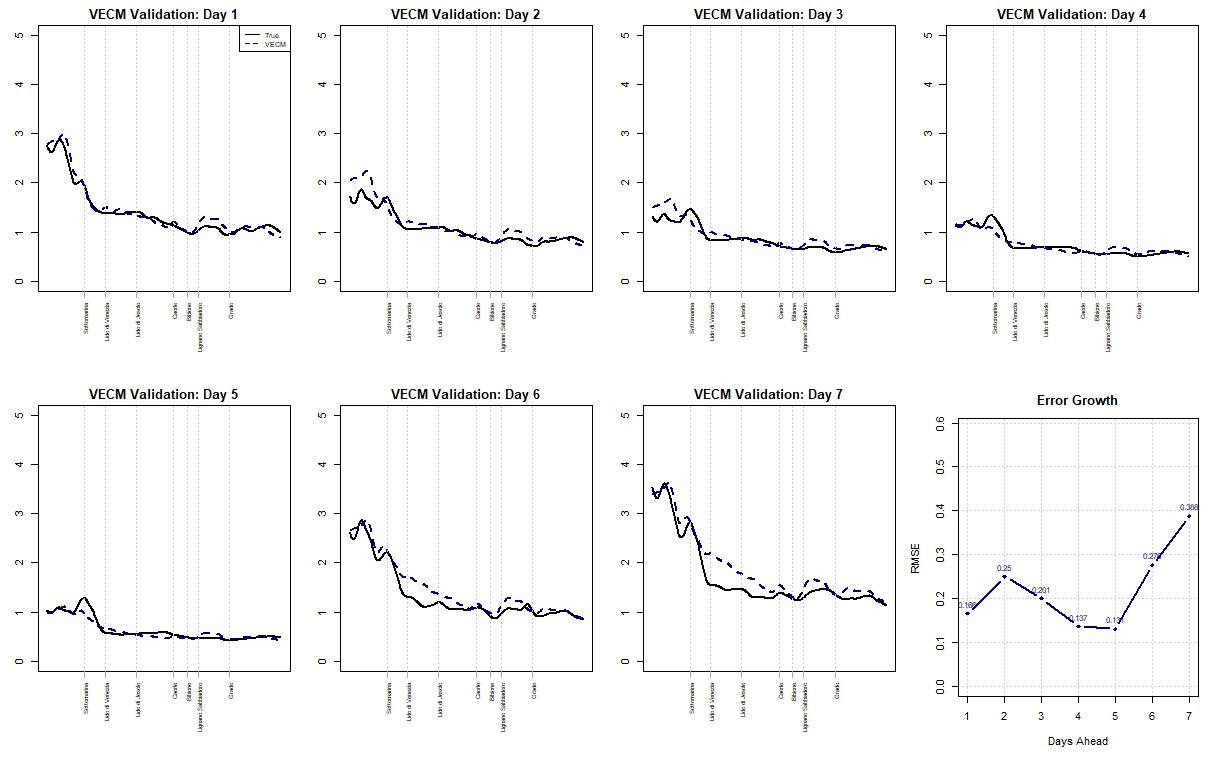
\includegraphics[width=0.8\textwidth]{Images/VECM validation giusto.jpeg}
    \caption{VECM validation plots.}
    \label{fig:VECM_validation}
\end{figure}

Figure \ref{fig:VECM_validation} illustrates the forecasting performance of the VECM over a 7-day horizon. The model successfully tracks the temporal evolution of the profiles, maintaining the physical consistency of the North-South gradient even during the final days of the window.

\subsection{Model Diagnostics and Residual Analysis}

To ensure the statistical validity of the selected VECM ($r=3$, $p=7$), we analyzed its residual series ($\hat{\varepsilon}_{t,1}, \dots, \hat{\varepsilon}_{t,4}$). A well-specified model should ideally yield residuals that behave as pure white noise.

The formal \textbf{Multivariate Portmanteau Test} returned a highly significant $p$-value ($< 0.001$), rejecting the hypothesis of perfect white noise. However, visual inspection of the AutoCorrelation Function (ACF) provides essential context.

\begin{figure}[h!]
    \centering
    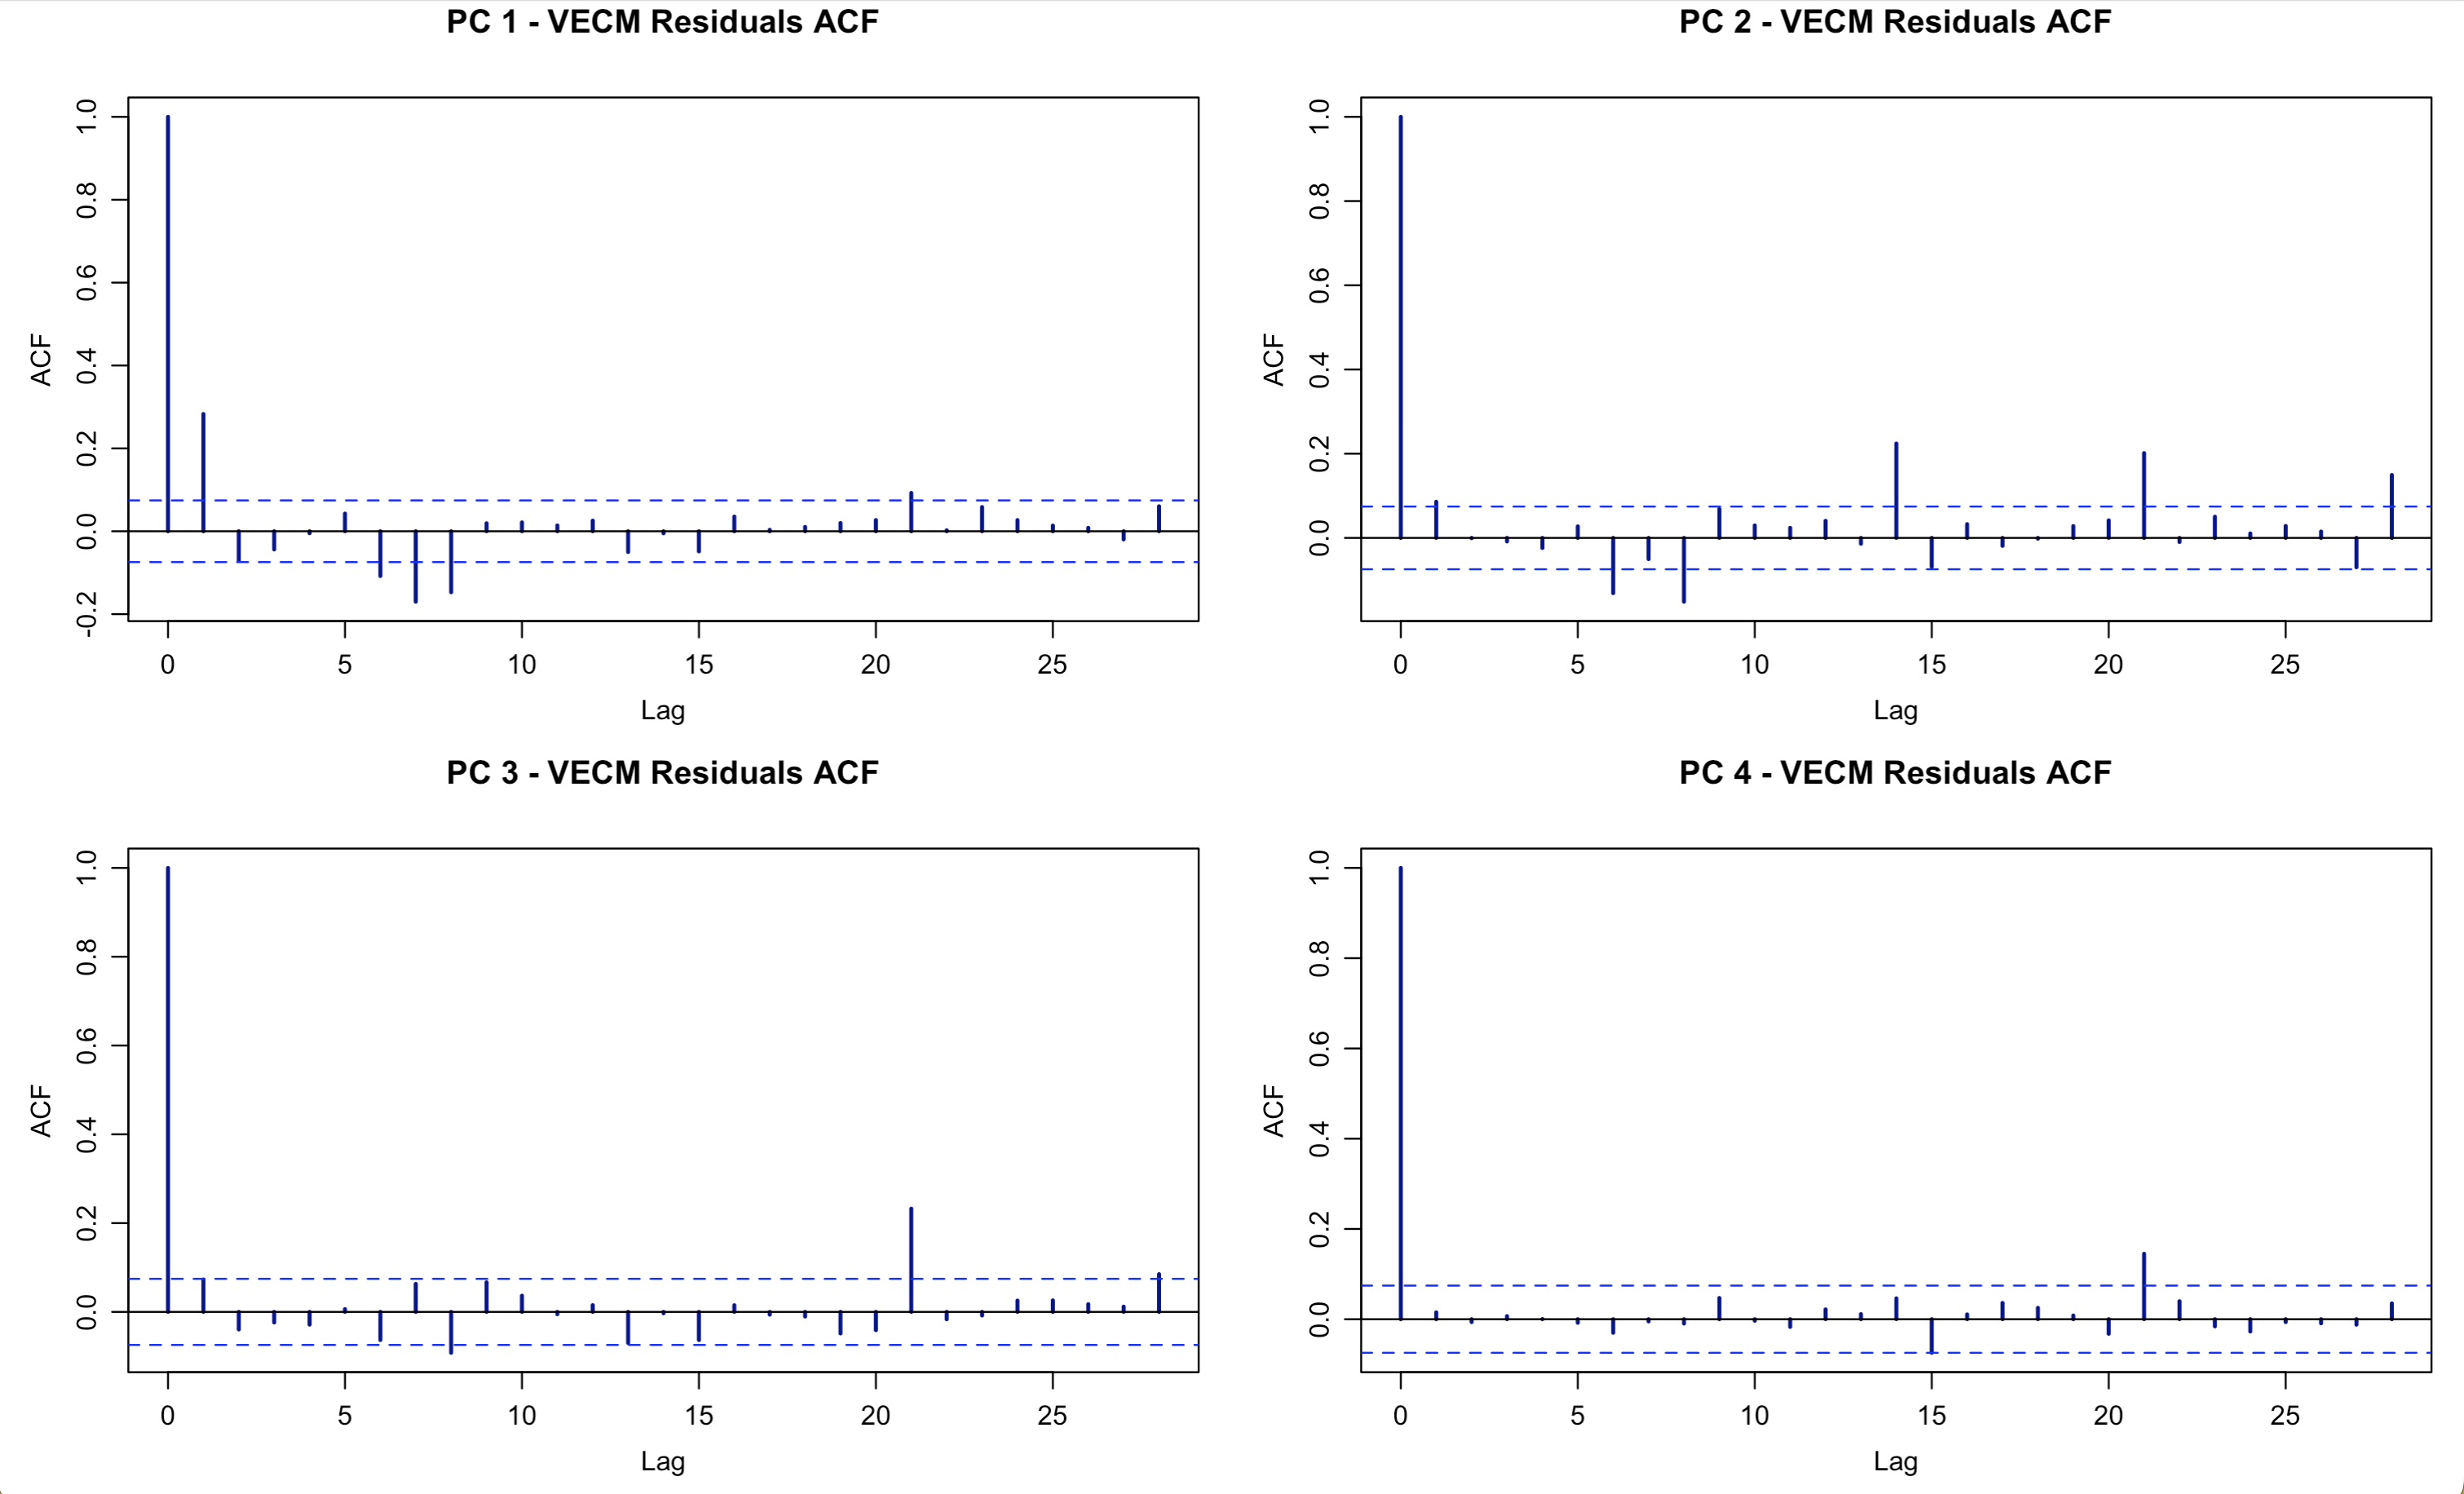
\includegraphics[width=0.8\textwidth]{Images/VECM reesiduals AFC.jpeg}
    \caption{VECM residuals AutoCorrelation Functions.}
    \label{fig:nome_etichetta}
\end{figure}

As shown in the ACF plots, the vast majority of residual autocorrelations fall safely within the $95\%$ Bartlett confidence bounds. The test's failure is primarily driven by minor, isolated spikes—an unavoidable artifact in noisy, high-frequency environmental data. 

This highlights a classic bias-variance tradeoff. While artificially increasing the lag order (e.g., to $p=14$) might "clean" the residuals and pass the formal test, it would simultaneously trigger the \textit{curse of dimensionality}, leading to severe overfitting and out-of-sample collapse. We therefore retained the parsimonious $p=7$ structure. 

Finally, distributional analysis confirmed that the residuals closely follow a zero-mean Gaussian profile. Together, these diagnostics validate the structural integrity of the VECM, confirming it as a robust operational forecasting engine.

\clearpage

\newpage
\newpage
\section{Uncertainty Quantification: Conformal Prediction}
\label{sec:conformal}

While the VECM provides accurate point forecasts, the inherent stochasticity of marine ecosystems—driven by sudden meteorological changes and nutrient discharges—requires a formal quantification of uncertainty. For \textit{Meteo.Adriatico}, a point forecast of "low chlorophyll" is only operationally useful if accompanied by a statistically rigorous "worst-case scenario" to manage tourist expectations. To provide these guarantees without assuming a specific parametric distribution for the forecast errors, we implemented a \textbf{Conformal Prediction (CP)} framework.

\subsection{The Challenge of Temporal Dependence}

Standard Inductive Conformal Prediction (ICP) typically relies on the assumption of \textit{exchangeability} (i.e., the joint distribution of the data is invariant under permutation). However, our Chlorophyll functions $X_t(d)$ exhibit strong \textbf{temporal autocorrelation} and non-stationarity, as evidenced by the seasonal clusters of outliers identified in Section \ref{subsec:outliers}. This deviation from exchangeability requires a strategic approach to calibration to ensure the validity of the predictive regions.

In this framework, the conformal regions are designed to satisfy a target confidence level of $1 - \alpha$. For this study, we set $\alpha = 0.05$, corresponding to a $95\%$ confidence rate. To construct these conformal bands, we utilized a \textbf{calibration set} consisting of $n_{cal} = 20$ days. This choice adheres to the empirical rule of thumb:
\begin{equation}
    n_{cal} \approx \frac{1}{\alpha}
\end{equation}
which, given our significance level, suggests that approximately $20$ samples are required to provide a stable estimate of the $1-\alpha$ quantile. Finally, the validation of the model's performance and the empirical coverage of the resulting bands were conducted using a \textbf{validation set} of $7$ days (one week), providing a representative window to assess the model's reliability over a standard short-term temporal horizon.

If a static calibration set were used, the resulting prediction bands would fail to adapt to shifting sea conditions (e.g., a sudden spring bloom increasing variance). To address this, we adopted \textbf{Adaptive Conformal Inference (ACI)} \cite{gibbs2021adaptive}. Unlike static CP, ACI updates the error quantiles dynamically: if the model under-predicts the observed value today, the "confidence budget" is adjusted to widen the bands for tomorrow. This ensures that the target coverage error $\alpha$ is maintained even under distribution shift and strong serial dependence.


\subsection{Defining the Conformal Score and Band Geometry}
We define our prediction interval for the functional curve at a future time $t+h$ as:
$$ \hat{C}_{t+h}(d) = [ \hat{X}_{t+h}(d) - q_t, \hat{X}_{t+h}(d) + q_t ] $$
where $\hat{X}_{t+h}(d)$ is the VECM-reconstructed curve and $q_t$ is the conformal score. In our functional context, $q_t$ is calculated based on the $L_\infty$ norm of past residuals, ensuring that the entire spatial profile is covered with a simultaneous probability of $1-\alpha$.

\subsection{Positivity Constraints and Log-Transform Strategy}
A primary challenge arose during the initial implementation: because Chlorophyll-a concentrations are strictly non-negative physical quantities ($Chl \geq 0$), the symmetric bands generated by linear CP often dipped below zero, especially during periods of high forecasted variance. 

While a simple \textbf{truncation} at zero ($\max(0, \hat{C}_{t+h})$) would prevent physical impossibility, it produces "pinched" asymmetric intervals that lose their formal probabilistic interpretation and fail to capture the heteroscedastic nature of algal growth. To resolve this, we performed the Conformal Inference on the \textbf{log-transformed} domain:
\begin{enumerate}
    \item \textbf{Transformation:} Map the historical data to $Y_t(d) = \log(X_t(d))$.
    \item \textbf{Estimation:} Compute VECM forecasts and ACI bands ($q_t^{log}$) in the log-space.
    \item \textbf{Back-transformation:} Project the intervals back to the original scale: 
    $$ \exp( \hat{Y}_{t+h}(d) \pm q_t^{log} ) $$
\end{enumerate}

This multiplicative approach ensures that the prediction bands are naturally bounded at zero ($e^x > 0$) and exhibit physically consistent behavior: the bands widen during massive bloom events (where uncertainty is higher) and narrow during clear-water periods. This provides \textit{Meteo.Adriatico} with a more ecologically sound risk assessment tool.

\begin{figure}[h!]
    \centering
    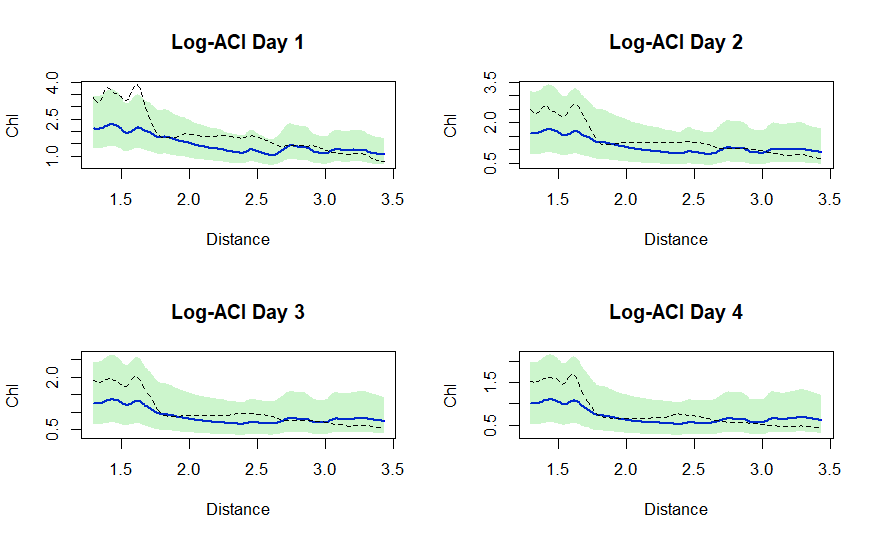
\includegraphics[width=0.8\textwidth]{Images/conformal_1.png}
    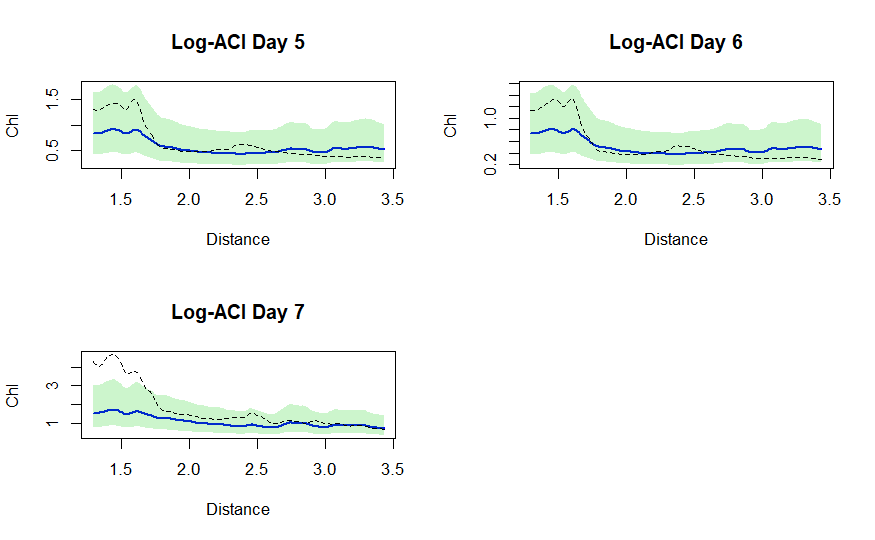
\includegraphics[width=0.8\textwidth]{Images/conformal_2.jpg}
    \caption{7-day functional forecast with $95\%$ Adaptive Conformal bands. The log-transformation ensures the lower bound remains strictly positive and adapts to the magnitude of the bloom.}
    \label{fig:conformal_results}
\end{figure}

\newpage
\section{Conclusions and Future Developments}
\label{sec:conclusions}

This project successfully established a functional forecasting framework for Chlorophyll-a concentrations along the Northern Adriatic coast. By integrating Functional Data Analysis (FDA) with multivariate time-series modeling, we moved beyond discrete spatial observations to a continuous, operationally relevant representation of the marine ecosystem for \textit{Meteo.Adriatico}.

\subsection{Final Remarks on Results}
The evaluation of the predictive pipeline yields several key insights into the behavior and predictability of the Adriatic coastline:
\begin{itemize}
    \item \textbf{Predictive Stability:} The transition from raw data to functional principal components allowed the models to filter out the ``weekly artifacts'' of the Copernicus reanalysis. Consequently, the VECM achieved a high degree of accuracy ($RMSE \approx 0.22$), successfully tracking the North-South gradient and seasonal shifts over a 7-day horizon.
    \item \textbf{Interdependence of Spatial Zones:} A critical finding was the existence of cointegration among the spatial modes of the coast. This suggests that the biological state of the Northern Adriatic does not evolve as a coupled system where different coastal segments share long-term equilibrium trends.
    \item \textbf{Reliability of the Worst-Case Scenario:} The implementation of Adaptive Conformal Inference (ACI) provided a significant upgrade from simple point forecasts. By performing inference in the log-domain, the model naturally produced uncertainty margins that are physically consistent ($Chl > 0$) and scale with the magnitude of the predicted bloom.
\end{itemize}

\subsection{Future Developments}
To evolve this tool from a statistical proxy into a high-fidelity marine digital twin, the following research directions are proposed:

\subsubsection{Deep Learning for Functional Sequence Prediction}
While the VECM captures linear cointegration, the sudden onset of algal blooms often exhibits non-linear threshold dynamics. Future work will explore replacing the VAR-based core with \textbf{Recurrent Neural Networks (RNNs)} or \textbf{Long Short-Term Memory (LSTM)} networks. By training an LSTM on the FPCA scores, the model can learn long-range temporal dependencies and non-linear interactions between spatial modes. Furthermore, a \textbf{Functional Neural Network} approach could be used to map the previous $p$ days of curves directly to the future curve $X_{t+h}(d)$, bypassing the limitations of linear dimensionality reduction.

\subsubsection{Expansion of the Multi-Source Data Reservoir}
The current model relies solely on Chlorophyll-a reanalysis. Increasing the predictive horizon and accuracy will require a multi-modal dataset. We propose integrating:
\begin{itemize}
    \item \textbf{Remote Sensing Reflectance (Rrs):} Direct satellite-derived optical data to bypass the numerical smoothing of reanalysis models.
    \item \textbf{Riverine Inputs:} Real-time discharge and nutrient concentration data from the \textbf{Po River Authority}, providing a 24-48 hour leading indicator of nutrient loading.
    \item \textbf{In-situ Sensors:} Integrating high-frequency data from coastal buoys to correct the drift of the functional profiles in real-time.
\end{itemize}

\subsubsection{Physics-Informed Neural Networks (PINNs)}
To ensure that forecasts do not merely follow statistical trends but respect the laws of fluid dynamics, we propose a \textbf{Physics-Informed} approach. By incorporating the \textbf{Advection-Diffusion-Reaction (ADR)} equations into the loss function of a Neural Network, we can constrain the predicted Chlorophyll concentration $C$ based on the velocity field of marine currents $\mathbf{u}$:
\begin{equation}
    \frac{\partial C}{\partial t} + \nabla \cdot (C\mathbf{u}) = \kappa \nabla^2 C + R(C)
\end{equation}
Where $\kappa$ is the diffusion coefficient and $R(C)$ represents the biological reaction term (growth and decay). This integration would allow the model to account for the transport of algal masses by \textbf{Adriatic surface currents}, such as the Western Adriatic Current (WAC), significantly improving the spatial accuracy of the forecast during storm events or shifts in circulation.

\newpage
\bibliographystyle{unsrt}
\bibliography{references}

\end{document}
